%%%%%%%% Preprint version in the Tencent Hunyuan technical-report template %%%%%%%%%%%%%%%%%
% Same content as example_paper.tex (ICML submission) through sections/*.tex.
% Template: tencent_hunyuan.sty / tencent_hunyuan.bst / logo/hunyuanlogo.png, taken from the LaTeX sources of
% HunyuanOCR (arXiv:2511.19575) and Hunyuan-TurboS (arXiv:2505.15431). The logo in the first-page header marks
% the report as a Tencent Hunyuan publication: confirm with the Tencent collaborators before posting.
% To drop the logo, comment out \lhead{...} in tencent_hunyuan.sty (fancypagestyle{firstpage}).

\documentclass{article}
\PassOptionsToPackage{table}{xcolor}
\usepackage{tencent_hunyuan}
\usepackage{caption}

% Unified table colors
\definecolor{tabGroup}{HTML}{E9EDF2}
\definecolor{tabFull}{HTML}{E6F0FC}
\definecolor{tabBest}{HTML}{E5F3E9}
\definecolor{tabOracle}{HTML}{FFF0DD}
\definecolor{tabMuted}{HTML}{697586}

\definecolor{tabHighlight}{HTML}{FFF0DD}

\definecolor{tabLoad}{HTML}{F1F4F8}
\definecolor{tabGain}{HTML}{E5F3E9}

\definecolor{tabDrop}{HTML}{FBE6E6}

% Scenario-specific column colors
\definecolor{tabCode}{HTML}{EAF2FB}
\definecolor{tabChinese}{HTML}{F2EEFA}
\definecolor{tabMoE}{HTML}{E9F4F1}
\definecolor{tabDrop}{HTML}{FBE6E6}

% Shared preamble for example_paper.tex (ICML) and pre.tex (Tencent template).
% Load after the template style. xcolor must already carry the [table] option (\PassOptionsToPackage before the style).
\usepackage{microtype}
\usepackage{graphicx}
\usepackage{booktabs}
\usepackage{tabularx}
\usepackage{array}
\usepackage{xcolor}
\usepackage{amsmath}
\usepackage{amssymb}
\usepackage{mathtools}
\usepackage{algorithm}
\usepackage{algorithmic}
\usepackage{tikz}
\usetikzlibrary{positioning,arrows.meta,calc,fit}
\usepackage{placeins}
\usepackage[capitalize,noabbrev]{cleveref}

% pages that hold only floats (appendix tables): stack from the top with fixed gaps instead of spreading them out
\makeatletter
\setlength{\@fptop}{0pt}
\setlength{\@fpsep}{14pt plus 4pt}
\setlength{\@fpbot}{0pt plus 1fil}
\makeatother

\definecolor{resultgray}{gray}{0.88}
\definecolor{resultgraylight}{gray}{0.93}

% table colours used by the hand-styled tables (shared by both versions)
\definecolor{tabGroup}{HTML}{E9EDF2}
\definecolor{tabFull}{HTML}{E6F0FC}
\definecolor{tabBest}{HTML}{E5F3E9}
\definecolor{tabOracle}{HTML}{FFF0DD}
\definecolor{tabMuted}{HTML}{697586}
\definecolor{tabHighlight}{HTML}{FFF0DD}
\definecolor{tabLoad}{HTML}{F1F4F8}
\definecolor{tabGain}{HTML}{E5F3E9}
\definecolor{tabDrop}{HTML}{FBE6E6}
\definecolor{tabCode}{HTML}{EAF2FB}
\definecolor{tabChinese}{HTML}{F2EEFA}
\definecolor{tabMoE}{HTML}{E9F4F1}

% every number in the text comes from numbers.tex, generated from the frozen data by
% code/specsched/paper_assets.py; a missing key prints ??key?? and raises a warning
% generated by code/specsched/paper_assets.py from the frozen data -- do not edit by hand
\providecommand{\nv}[1]{\ifcsname nv@#1\endcsname\csname nv@#1\endcsname\else\textbf{??#1??}\GenericWarning{}{LaTeX Warning: missing number #1}\fi}
\expandafter\def\csname nv@code.best\endcsname{Informed schedule}
\expandafter\def\csname nv@code.prod.thr\endcsname{14{,}601}
\expandafter\def\csname nv@code.prod.r\endcsname{0.854}
\expandafter\def\csname nv@code.prod.short\endcsname{14.6}
\expandafter\def\csname nv@code.prod.d\endcsname{$+2.2$}
\expandafter\def\csname nv@code.prod.sd\endcsname{0.9}
\expandafter\def\csname nv@code.prod.abs\endcsname{2.2}
\expandafter\def\csname nv@code.static.thr\endcsname{14{,}282}
\expandafter\def\csname nv@code.static.r\endcsname{0.835}
\expandafter\def\csname nv@code.static.short\endcsname{16.5}
\expandafter\def\csname nv@code.plain.thr\endcsname{16{,}869}
\expandafter\def\csname nv@code.plain.r\endcsname{0.986}
\expandafter\def\csname nv@code.plain.short\endcsname{1.4}
\expandafter\def\csname nv@code.plain.d\endcsname{$+18.1$}
\expandafter\def\csname nv@code.plain.sd\endcsname{0.9}
\expandafter\def\csname nv@code.plain.abs\endcsname{18.1}
\expandafter\def\csname nv@code.switch.thr\endcsname{16{,}120}
\expandafter\def\csname nv@code.switch.r\endcsname{0.943}
\expandafter\def\csname nv@code.switch.short\endcsname{5.7}
\expandafter\def\csname nv@code.switch.d\endcsname{$+12.9$}
\expandafter\def\csname nv@code.switch.sd\endcsname{2.5}
\expandafter\def\csname nv@code.switch.abs\endcsname{12.9}
\expandafter\def\csname nv@code.thresh.thr\endcsname{16{,}400}
\expandafter\def\csname nv@code.thresh.r\endcsname{0.959}
\expandafter\def\csname nv@code.thresh.short\endcsname{4.1}
\expandafter\def\csname nv@code.thresh.d\endcsname{$+14.8$}
\expandafter\def\csname nv@code.thresh.sd\endcsname{0.8}
\expandafter\def\csname nv@code.thresh.abs\endcsname{14.8}
\expandafter\def\csname nv@code.tide.thr\endcsname{16{,}253}
\expandafter\def\csname nv@code.tide.r\endcsname{0.950}
\expandafter\def\csname nv@code.tide.short\endcsname{5.0}
\expandafter\def\csname nv@code.tide.d\endcsname{$+13.8$}
\expandafter\def\csname nv@code.tide.sd\endcsname{3.5}
\expandafter\def\csname nv@code.tide.abs\endcsname{13.8}
\expandafter\def\csname nv@code.always.thr\endcsname{14{,}617}
\expandafter\def\csname nv@code.always.r\endcsname{0.855}
\expandafter\def\csname nv@code.always.short\endcsname{14.5}
\expandafter\def\csname nv@code.always.d\endcsname{$+2.4$}
\expandafter\def\csname nv@code.always.sd\endcsname{1.9}
\expandafter\def\csname nv@code.always.abs\endcsname{2.4}
\expandafter\def\csname nv@code.informed.thr\endcsname{17{,}102}
\expandafter\def\csname nv@code.informed.r\endcsname{1.000}
\expandafter\def\csname nv@code.informed.short\endcsname{0.0}
\expandafter\def\csname nv@code.informed.d\endcsname{$+19.7$}
\expandafter\def\csname nv@code.informed.sd\endcsname{0.5}
\expandafter\def\csname nv@code.informed.abs\endcsname{19.7}
\expandafter\def\csname nv@code.full.thr\endcsname{16{,}853}
\expandafter\def\csname nv@code.full.r\endcsname{0.985}
\expandafter\def\csname nv@code.full.short\endcsname{1.5}
\expandafter\def\csname nv@code.full.d\endcsname{$+18.0$}
\expandafter\def\csname nv@code.full.sd\endcsname{1.6}
\expandafter\def\csname nv@code.full.abs\endcsname{18.0}
\expandafter\def\csname nv@zh.best\endcsname{Plain decoding}
\expandafter\def\csname nv@zh.prod.thr\endcsname{8{,}682}
\expandafter\def\csname nv@zh.prod.r\endcsname{0.517}
\expandafter\def\csname nv@zh.prod.short\endcsname{48.3}
\expandafter\def\csname nv@zh.prod.d\endcsname{$+1.8$}
\expandafter\def\csname nv@zh.prod.sd\endcsname{0.8}
\expandafter\def\csname nv@zh.prod.abs\endcsname{1.8}
\expandafter\def\csname nv@zh.static.thr\endcsname{8{,}526}
\expandafter\def\csname nv@zh.static.r\endcsname{0.508}
\expandafter\def\csname nv@zh.static.short\endcsname{49.2}
\expandafter\def\csname nv@zh.plain.thr\endcsname{16{,}794}
\expandafter\def\csname nv@zh.plain.r\endcsname{1.000}
\expandafter\def\csname nv@zh.plain.short\endcsname{0.0}
\expandafter\def\csname nv@zh.plain.d\endcsname{$+97.0$}
\expandafter\def\csname nv@zh.plain.sd\endcsname{1.4}
\expandafter\def\csname nv@zh.plain.abs\endcsname{97.0}
\expandafter\def\csname nv@zh.switch.thr\endcsname{16{,}273}
\expandafter\def\csname nv@zh.switch.r\endcsname{0.969}
\expandafter\def\csname nv@zh.switch.short\endcsname{3.1}
\expandafter\def\csname nv@zh.switch.d\endcsname{$+90.9$}
\expandafter\def\csname nv@zh.switch.sd\endcsname{2.2}
\expandafter\def\csname nv@zh.switch.abs\endcsname{90.9}
\expandafter\def\csname nv@zh.thresh.thr\endcsname{15{,}936}
\expandafter\def\csname nv@zh.thresh.r\endcsname{0.949}
\expandafter\def\csname nv@zh.thresh.short\endcsname{5.1}
\expandafter\def\csname nv@zh.thresh.d\endcsname{$+86.9$}
\expandafter\def\csname nv@zh.thresh.sd\endcsname{4.7}
\expandafter\def\csname nv@zh.thresh.abs\endcsname{86.9}
\expandafter\def\csname nv@zh.tide.thr\endcsname{13{,}170}
\expandafter\def\csname nv@zh.tide.r\endcsname{0.784}
\expandafter\def\csname nv@zh.tide.short\endcsname{21.6}
\expandafter\def\csname nv@zh.tide.d\endcsname{$+54.5$}
\expandafter\def\csname nv@zh.tide.sd\endcsname{3.6}
\expandafter\def\csname nv@zh.tide.abs\endcsname{54.5}
\expandafter\def\csname nv@zh.always.thr\endcsname{8{,}427}
\expandafter\def\csname nv@zh.always.r\endcsname{0.502}
\expandafter\def\csname nv@zh.always.short\endcsname{49.8}
\expandafter\def\csname nv@zh.always.d\endcsname{$-1.2$}
\expandafter\def\csname nv@zh.always.sd\endcsname{0.7}
\expandafter\def\csname nv@zh.always.abs\endcsname{1.2}
\expandafter\def\csname nv@zh.informed.thr\endcsname{9{,}699}
\expandafter\def\csname nv@zh.informed.r\endcsname{0.578}
\expandafter\def\csname nv@zh.informed.short\endcsname{42.2}
\expandafter\def\csname nv@zh.informed.d\endcsname{$+13.8$}
\expandafter\def\csname nv@zh.informed.sd\endcsname{0.4}
\expandafter\def\csname nv@zh.informed.abs\endcsname{13.8}
\expandafter\def\csname nv@zh.full.thr\endcsname{15{,}997}
\expandafter\def\csname nv@zh.full.r\endcsname{0.953}
\expandafter\def\csname nv@zh.full.short\endcsname{4.7}
\expandafter\def\csname nv@zh.full.d\endcsname{$+87.7$}
\expandafter\def\csname nv@zh.full.sd\endcsname{8.5}
\expandafter\def\csname nv@zh.full.abs\endcsname{87.7}
\expandafter\def\csname nv@moe.best\endcsname{Informed schedule}
\expandafter\def\csname nv@moe.prod.thr\endcsname{13{,}992}
\expandafter\def\csname nv@moe.prod.r\endcsname{0.923}
\expandafter\def\csname nv@moe.prod.short\endcsname{7.7}
\expandafter\def\csname nv@moe.prod.d\endcsname{$+1.0$}
\expandafter\def\csname nv@moe.prod.sd\endcsname{0.1}
\expandafter\def\csname nv@moe.prod.abs\endcsname{1.0}
\expandafter\def\csname nv@moe.static.thr\endcsname{13{,}859}
\expandafter\def\csname nv@moe.static.r\endcsname{0.915}
\expandafter\def\csname nv@moe.static.short\endcsname{8.5}
\expandafter\def\csname nv@moe.plain.thr\endcsname{7{,}465}
\expandafter\def\csname nv@moe.plain.r\endcsname{0.493}
\expandafter\def\csname nv@moe.plain.short\endcsname{50.7}
\expandafter\def\csname nv@moe.plain.d\endcsname{$-46.1$}
\expandafter\def\csname nv@moe.plain.sd\endcsname{0.1}
\expandafter\def\csname nv@moe.plain.abs\endcsname{46.1}
\expandafter\def\csname nv@moe.switch.thr\endcsname{13{,}816}
\expandafter\def\csname nv@moe.switch.r\endcsname{0.912}
\expandafter\def\csname nv@moe.switch.short\endcsname{8.8}
\expandafter\def\csname nv@moe.switch.d\endcsname{$-0.3$}
\expandafter\def\csname nv@moe.switch.sd\endcsname{0.3}
\expandafter\def\csname nv@moe.switch.abs\endcsname{0.3}
\expandafter\def\csname nv@moe.thresh.thr\endcsname{7{,}489}
\expandafter\def\csname nv@moe.thresh.r\endcsname{0.494}
\expandafter\def\csname nv@moe.thresh.short\endcsname{50.6}
\expandafter\def\csname nv@moe.thresh.d\endcsname{$-46.0$}
\expandafter\def\csname nv@moe.thresh.sd\endcsname{0.0}
\expandafter\def\csname nv@moe.thresh.abs\endcsname{46.0}
\expandafter\def\csname nv@moe.tide.thr\endcsname{14{,}692}
\expandafter\def\csname nv@moe.tide.r\endcsname{0.970}
\expandafter\def\csname nv@moe.tide.short\endcsname{3.0}
\expandafter\def\csname nv@moe.tide.d\endcsname{$+6.0$}
\expandafter\def\csname nv@moe.tide.sd\endcsname{4.0}
\expandafter\def\csname nv@moe.tide.abs\endcsname{6.0}
\expandafter\def\csname nv@moe.always.thr\endcsname{13{,}364}
\expandafter\def\csname nv@moe.always.r\endcsname{0.882}
\expandafter\def\csname nv@moe.always.short\endcsname{11.8}
\expandafter\def\csname nv@moe.always.d\endcsname{$-3.6$}
\expandafter\def\csname nv@moe.always.sd\endcsname{0.3}
\expandafter\def\csname nv@moe.always.abs\endcsname{3.6}
\expandafter\def\csname nv@moe.informed.thr\endcsname{15{,}151}
\expandafter\def\csname nv@moe.informed.r\endcsname{1.000}
\expandafter\def\csname nv@moe.informed.short\endcsname{0.0}
\expandafter\def\csname nv@moe.informed.d\endcsname{$+9.3$}
\expandafter\def\csname nv@moe.informed.sd\endcsname{0.7}
\expandafter\def\csname nv@moe.informed.abs\endcsname{9.3}
\expandafter\def\csname nv@moe.full.thr\endcsname{14{,}967}
\expandafter\def\csname nv@moe.full.r\endcsname{0.988}
\expandafter\def\csname nv@moe.full.short\endcsname{1.2}
\expandafter\def\csname nv@moe.full.d\endcsname{$+8.0$}
\expandafter\def\csname nv@moe.full.sd\endcsname{0.4}
\expandafter\def\csname nv@moe.full.abs\endcsname{8.0}
\expandafter\def\csname nv@prod.worst\endcsname{0.517}
\expandafter\def\csname nv@prod.worstshort\endcsname{48.3}
\expandafter\def\csname nv@static.worst\endcsname{0.508}
\expandafter\def\csname nv@static.worstshort\endcsname{49.2}
\expandafter\def\csname nv@plain.worst\endcsname{0.493}
\expandafter\def\csname nv@plain.worstshort\endcsname{50.7}
\expandafter\def\csname nv@switch.worst\endcsname{0.912}
\expandafter\def\csname nv@switch.worstshort\endcsname{8.8}
\expandafter\def\csname nv@thresh.worst\endcsname{0.494}
\expandafter\def\csname nv@thresh.worstshort\endcsname{50.6}
\expandafter\def\csname nv@tide.worst\endcsname{0.784}
\expandafter\def\csname nv@tide.worstshort\endcsname{21.6}
\expandafter\def\csname nv@always.worst\endcsname{0.502}
\expandafter\def\csname nv@always.worstshort\endcsname{49.8}
\expandafter\def\csname nv@informed.worst\endcsname{0.578}
\expandafter\def\csname nv@informed.worstshort\endcsname{42.2}
\expandafter\def\csname nv@full.worst\endcsname{0.953}
\expandafter\def\csname nv@full.worstshort\endcsname{4.7}
\expandafter\def\csname nv@others.maxworst\endcsname{0.784}
\expandafter\def\csname nv@alt.minshort\endcsname{8.8}
\expandafter\def\csname nv@alt.minshort.floor\endcsname{8}
\expandafter\def\csname nv@alt.best\endcsname{Switch only}
\expandafter\def\csname nv@others.minshortfall\endcsname{22}
\expandafter\def\csname nv@code.full.p99\endcsname{$-5.1$}
\expandafter\def\csname nv@code.full.a2\endcsname{$-1.8$}
\expandafter\def\csname nv@code.full.a1\endcsname{$+10.1$}
\expandafter\def\csname nv@code.full.session\endcsname{$+10.9$}
\expandafter\def\csname nv@code.full.sessionsd\endcsname{1.1}
\expandafter\def\csname nv@code.informed.a2\endcsname{$-16.4$}
\expandafter\def\csname nv@zh.full.p99\endcsname{$-49.5$}
\expandafter\def\csname nv@zh.full.a2\endcsname{$+2.8$}
\expandafter\def\csname nv@zh.full.a1\endcsname{$+11.6$}
\expandafter\def\csname nv@zh.full.session\endcsname{$+67.3$}
\expandafter\def\csname nv@zh.full.sessionsd\endcsname{5.3}
\expandafter\def\csname nv@zh.informed.a2\endcsname{$-11.1$}
\expandafter\def\csname nv@moe.full.p99\endcsname{$-3.6$}
\expandafter\def\csname nv@moe.full.a2\endcsname{$-9.5$}
\expandafter\def\csname nv@moe.full.a1\endcsname{$-0.8$}
\expandafter\def\csname nv@moe.full.session\endcsname{$+6.5$}
\expandafter\def\csname nv@moe.full.sessionsd\endcsname{0.3}
\expandafter\def\csname nv@moe.informed.a2\endcsname{$-8.1$}
\expandafter\def\csname nv@code.full_vs_switch\endcsname{$+4.6$}
\expandafter\def\csname nv@code.full_vs_switch.sd\endcsname{2.5}
\expandafter\def\csname nv@code.full_vs_plain\endcsname{$-0.1$}
\expandafter\def\csname nv@code.full_vs_informed\endcsname{$-1.5$}
\expandafter\def\csname nv@code.full_vs_informed.min\endcsname{$-2.5$}
\expandafter\def\csname nv@code.full_vs_informed.max\endcsname{$+0.5$}
\expandafter\def\csname nv@code.full_vs_informed.samesign\endcsname{no}
\expandafter\def\csname nv@code.full_vs_thresh\endcsname{$+2.8$}
\expandafter\def\csname nv@zh.full_vs_switch\endcsname{$-1.7$}
\expandafter\def\csname nv@zh.full_vs_switch.sd\endcsname{3.6}
\expandafter\def\csname nv@zh.full_vs_plain\endcsname{$-4.7$}
\expandafter\def\csname nv@zh.full_vs_informed\endcsname{$+65.0$}
\expandafter\def\csname nv@zh.full_vs_informed.min\endcsname{$+56.4$}
\expandafter\def\csname nv@zh.full_vs_informed.max\endcsname{$+71.2$}
\expandafter\def\csname nv@zh.full_vs_informed.samesign\endcsname{yes}
\expandafter\def\csname nv@zh.full_vs_thresh\endcsname{$+0.4$}
\expandafter\def\csname nv@moe.full_vs_switch\endcsname{$+8.3$}
\expandafter\def\csname nv@moe.full_vs_switch.sd\endcsname{0.7}
\expandafter\def\csname nv@moe.full_vs_plain\endcsname{$+100.5$}
\expandafter\def\csname nv@moe.full_vs_informed\endcsname{$-1.2$}
\expandafter\def\csname nv@moe.full_vs_informed.min\endcsname{$-1.7$}
\expandafter\def\csname nv@moe.full_vs_informed.max\endcsname{$-0.9$}
\expandafter\def\csname nv@moe.full_vs_informed.samesign\endcsname{yes}
\expandafter\def\csname nv@moe.full_vs_thresh\endcsname{$+99.9$}
\expandafter\def\csname nv@code.switch_vs_plain\endcsname{$-4.4$}
\expandafter\def\csname nv@code.switch_vs_plain.abs\endcsname{4.4}
\expandafter\def\csname nv@zh.switch_vs_plain\endcsname{$-3.1$}
\expandafter\def\csname nv@zh.switch_vs_plain.abs\endcsname{3.1}
\expandafter\def\csname nv@code.infra\endcsname{2.2}
\expandafter\def\csname nv@zh.infra\endcsname{1.8}
\expandafter\def\csname nv@moe.infra\endcsname{1.0}
\expandafter\def\csname nv@n.runs\endcsname{81}
\expandafter\def\csname nv@n.pol\endcsname{nine}
\expandafter\def\csname nv@n.polcap\endcsname{Nine}
\expandafter\def\csname nv@gpuh\endcsname{27.4}
\expandafter\def\csname nv@gpuh.matrix\endcsname{19.8}
\expandafter\def\csname nv@cv.static.max\endcsname{0.7}
\expandafter\def\csname nv@cv.full.code\endcsname{1.1}
\expandafter\def\csname nv@cv.full.zh\endcsname{3.9}
\expandafter\def\csname nv@cv.full.moe\endcsname{0.3}
\expandafter\def\csname nv@cv.rule.min\endcsname{0.4}
\expandafter\def\csname nv@cv.rule.max\endcsname{2.7}
\expandafter\def\csname nv@bdur.min\endcsname{258}
\expandafter\def\csname nv@bdur.max\endcsname{600}
\expandafter\def\csname nv@hosts\endcsname{7}
\expandafter\def\csname nv@code.full.spec\endcsname{100}
\expandafter\def\csname nv@code.full.duty\endcsname{0.067}
\expandafter\def\csname nv@code.full.swaps\endcsname{3}
\expandafter\def\csname nv@code.full.acc0\endcsname{2.50}
\expandafter\def\csname nv@code.full.acc1\endcsname{2.66}
\expandafter\def\csname nv@code.full.tok\endcsname{0.64}
\expandafter\def\csname nv@code.full.why.saturated_no_value\endcsname{77}
\expandafter\def\csname nv@code.full.why.saturated_value\endcsname{10}
\expandafter\def\csname nv@code.full.why.converged\endcsname{10}
\expandafter\def\csname nv@code.full.why.free_within_slo\endcsname{2}
\expandafter\def\csname nv@code.full.why.at_ceiling\endcsname{1}
\expandafter\def\csname nv@code.full.why.no_slo_room\endcsname{0}
\expandafter\def\csname nv@zh.full.spec\endcsname{2}
\expandafter\def\csname nv@zh.full.duty\endcsname{0.016}
\expandafter\def\csname nv@zh.full.swaps\endcsname{1}
\expandafter\def\csname nv@zh.full.acc0\endcsname{1.18}
\expandafter\def\csname nv@zh.full.acc1\endcsname{1.18}
\expandafter\def\csname nv@zh.full.tok\endcsname{0.38}
\expandafter\def\csname nv@zh.full.why.structural_ceiling\endcsname{97}
\expandafter\def\csname nv@zh.full.why.free_within_slo\endcsname{2}
\expandafter\def\csname nv@zh.full.why.at_ceiling\endcsname{1}
\expandafter\def\csname nv@moe.full.spec\endcsname{100}
\expandafter\def\csname nv@moe.full.duty\endcsname{0.084}
\expandafter\def\csname nv@moe.full.swaps\endcsname{4}
\expandafter\def\csname nv@moe.full.acc0\endcsname{2.68}
\expandafter\def\csname nv@moe.full.acc1\endcsname{2.97}
\expandafter\def\csname nv@moe.full.tok\endcsname{0.81}
\expandafter\def\csname nv@moe.full.why.at_ceiling\endcsname{43}
\expandafter\def\csname nv@moe.full.why.saturated_no_value\endcsname{36}
\expandafter\def\csname nv@moe.full.why.saturated_value\endcsname{19}
\expandafter\def\csname nv@moe.full.why.converged\endcsname{1}
\expandafter\def\csname nv@moe.full.why.free_within_slo\endcsname{1}
\expandafter\def\csname nv@full.tok.max\endcsname{0.8}
\expandafter\def\csname nv@code.tide.rej\endcsname{3}
\expandafter\def\csname nv@code.tide.rejdrift\endcsname{0}
\expandafter\def\csname nv@code.tide.rounds\endcsname{8}
\expandafter\def\csname nv@code.tide.kept\endcsname{4.7}
\expandafter\def\csname nv@code.tide.rejected\endcsname{1.7}
\expandafter\def\csname nv@code.tide.drift\endcsname{1.7}
\expandafter\def\csname nv@code.tide.trainB\endcsname{38}
\expandafter\def\csname nv@code.tide.trainall\endcsname{56}
\expandafter\def\csname nv@code.tide.duty\endcsname{0.106}
\expandafter\def\csname nv@code.tide.spec\endcsname{100}
\expandafter\def\csname nv@code.tide.tok\endcsname{1.25}
\expandafter\def\csname nv@code.tide.acc1\endcsname{2.69}
\expandafter\def\csname nv@code.full_vs_tide\endcsname{$+3.7$}
\expandafter\def\csname nv@code.full_vs_tide.min\endcsname{$+1.9$}
\expandafter\def\csname nv@code.full_vs_tide.max\endcsname{$+5.7$}
\expandafter\def\csname nv@code.tide_vs_switch\endcsname{$+0.8$}
\expandafter\def\csname nv@code.tide_vs_switch.min\endcsname{$-1.8$}
\expandafter\def\csname nv@code.tide_vs_switch.max\endcsname{$+3.5$}
\expandafter\def\csname nv@code.tide_vs_informed\endcsname{$-5.0$}
\expandafter\def\csname nv@code.tide_vs_informed.min\endcsname{$-7.7$}
\expandafter\def\csname nv@code.tide_vs_informed.max\endcsname{$-1.4$}
\expandafter\def\csname nv@code.tide.a1\endcsname{$+12.1$}
\expandafter\def\csname nv@code.tide.a2\endcsname{$-0.8$}
\expandafter\def\csname nv@zh.tide.rej\endcsname{9}
\expandafter\def\csname nv@zh.tide.rejdrift\endcsname{7}
\expandafter\def\csname nv@zh.tide.rounds\endcsname{8}
\expandafter\def\csname nv@zh.tide.kept\endcsname{4.3}
\expandafter\def\csname nv@zh.tide.rejected\endcsname{3.0}
\expandafter\def\csname nv@zh.tide.drift\endcsname{2.3}
\expandafter\def\csname nv@zh.tide.trainB\endcsname{70}
\expandafter\def\csname nv@zh.tide.trainall\endcsname{70}
\expandafter\def\csname nv@zh.tide.duty\endcsname{0.299}
\expandafter\def\csname nv@zh.tide.spec\endcsname{16}
\expandafter\def\csname nv@zh.tide.tok\endcsname{0.53}
\expandafter\def\csname nv@zh.tide.acc1\endcsname{1.35}
\expandafter\def\csname nv@zh.full_vs_tide\endcsname{$+21.6$}
\expandafter\def\csname nv@zh.full_vs_tide.min\endcsname{$+12.7$}
\expandafter\def\csname nv@zh.full_vs_tide.max\endcsname{$+28.7$}
\expandafter\def\csname nv@zh.tide_vs_switch\endcsname{$-19.1$}
\expandafter\def\csname nv@zh.tide_vs_switch.min\endcsname{$-22.0$}
\expandafter\def\csname nv@zh.tide_vs_switch.max\endcsname{$-16.5$}
\expandafter\def\csname nv@zh.tide_vs_informed\endcsname{$+35.8$}
\expandafter\def\csname nv@zh.tide_vs_informed.min\endcsname{$+33.0$}
\expandafter\def\csname nv@zh.tide_vs_informed.max\endcsname{$+38.8$}
\expandafter\def\csname nv@zh.tide.a1\endcsname{$+13.1$}
\expandafter\def\csname nv@zh.tide.a2\endcsname{$-5.8$}
\expandafter\def\csname nv@moe.tide.rej\endcsname{3}
\expandafter\def\csname nv@moe.tide.rejdrift\endcsname{0}
\expandafter\def\csname nv@moe.tide.rounds\endcsname{4}
\expandafter\def\csname nv@moe.tide.kept\endcsname{1.0}
\expandafter\def\csname nv@moe.tide.rejected\endcsname{2.0}
\expandafter\def\csname nv@moe.tide.drift\endcsname{2.0}
\expandafter\def\csname nv@moe.tide.trainB\endcsname{26}
\expandafter\def\csname nv@moe.tide.trainall\endcsname{50}
\expandafter\def\csname nv@moe.tide.duty\endcsname{0.038}
\expandafter\def\csname nv@moe.tide.spec\endcsname{100}
\expandafter\def\csname nv@moe.tide.tok\endcsname{0.72}
\expandafter\def\csname nv@moe.tide.acc1\endcsname{2.92}
\expandafter\def\csname nv@moe.full_vs_tide\endcsname{$+2.0$}
\expandafter\def\csname nv@moe.full_vs_tide.min\endcsname{$-1.0$}
\expandafter\def\csname nv@moe.full_vs_tide.max\endcsname{$+5.8$}
\expandafter\def\csname nv@moe.tide_vs_switch\endcsname{$+6.3$}
\expandafter\def\csname nv@moe.tide_vs_switch.min\endcsname{$+1.9$}
\expandafter\def\csname nv@moe.tide_vs_switch.max\endcsname{$+10.2$}
\expandafter\def\csname nv@moe.tide_vs_informed\endcsname{$-3.0$}
\expandafter\def\csname nv@moe.tide_vs_informed.min\endcsname{$-6.3$}
\expandafter\def\csname nv@moe.tide_vs_informed.max\endcsname{$-0.1$}
\expandafter\def\csname nv@moe.tide.a1\endcsname{$+3.8$}
\expandafter\def\csname nv@moe.tide.a2\endcsname{$-4.2$}
\expandafter\def\csname nv@tide.noise.m1\endcsname{0.03}
\expandafter\def\csname nv@tide.noise.m1.n\endcsname{1{,}059}
\expandafter\def\csname nv@tide.noise.m2\endcsname{0.03}
\expandafter\def\csname nv@tide.noise.m2.n\endcsname{2{,}042}
\expandafter\def\csname nv@tide.roundgain.max\endcsname{0.03}
\expandafter\def\csname nv@tv.round\endcsname{800}
\expandafter\def\csname nv@tv.eps\endcsname{0.3}
\expandafter\def\csname nv@code.tv.thr\endcsname{16{,}514}
\expandafter\def\csname nv@code.tv.r\endcsname{0.966}
\expandafter\def\csname nv@code.full_vs_tv\endcsname{$+2.1$}
\expandafter\def\csname nv@code.full_vs_tv.min\endcsname{$+1.5$}
\expandafter\def\csname nv@code.full_vs_tv.max\endcsname{$+2.9$}
\expandafter\def\csname nv@code.full_vs_tv.samesign\endcsname{yes}
\expandafter\def\csname nv@code.tv_vs_tide\endcsname{$+1.7$}
\expandafter\def\csname nv@code.tv_vs_tide.min\endcsname{$-0.9$}
\expandafter\def\csname nv@code.tv_vs_tide.max\endcsname{$+4.1$}
\expandafter\def\csname nv@code.tv_vs_tide.samesign\endcsname{no}
\expandafter\def\csname nv@code.tv.trainB\endcsname{47}
\expandafter\def\csname nv@code.tv.rounds\endcsname{3.0}
\expandafter\def\csname nv@code.tv.drift\endcsname{1.0}
\expandafter\def\csname nv@code.tv.rej\endcsname{3}
\expandafter\def\csname nv@code.tv.rejdrift\endcsname{0}
\expandafter\def\csname nv@code.tv.norej\endcsname{0}
\expandafter\def\csname nv@zh.tv.thr\endcsname{14{,}484}
\expandafter\def\csname nv@zh.tv.r\endcsname{0.862}
\expandafter\def\csname nv@zh.full_vs_tv\endcsname{$+10.7$}
\expandafter\def\csname nv@zh.full_vs_tv.min\endcsname{$+2.2$}
\expandafter\def\csname nv@zh.full_vs_tv.max\endcsname{$+19.1$}
\expandafter\def\csname nv@zh.full_vs_tv.samesign\endcsname{yes}
\expandafter\def\csname nv@zh.tv_vs_tide\endcsname{$+10.0$}
\expandafter\def\csname nv@zh.tv_vs_tide.min\endcsname{$+8.1$}
\expandafter\def\csname nv@zh.tv_vs_tide.max\endcsname{$+11.5$}
\expandafter\def\csname nv@zh.tv_vs_tide.samesign\endcsname{yes}
\expandafter\def\csname nv@zh.tv.trainB\endcsname{51}
\expandafter\def\csname nv@zh.tv.rounds\endcsname{3.3}
\expandafter\def\csname nv@zh.tv.drift\endcsname{0.0}
\expandafter\def\csname nv@zh.tv.rej\endcsname{3}
\expandafter\def\csname nv@zh.tv.rejdrift\endcsname{0}
\expandafter\def\csname nv@zh.tv.norej\endcsname{0}
\expandafter\def\csname nv@moe.tv.thr\endcsname{14{,}887}
\expandafter\def\csname nv@moe.tv.r\endcsname{0.983}
\expandafter\def\csname nv@moe.full_vs_tv\endcsname{$+0.5$}
\expandafter\def\csname nv@moe.full_vs_tv.min\endcsname{$-0.2$}
\expandafter\def\csname nv@moe.full_vs_tv.max\endcsname{$+1.0$}
\expandafter\def\csname nv@moe.full_vs_tv.samesign\endcsname{no}
\expandafter\def\csname nv@moe.tv_vs_tide\endcsname{$+1.4$}
\expandafter\def\csname nv@moe.tv_vs_tide.min\endcsname{$-1.9$}
\expandafter\def\csname nv@moe.tv_vs_tide.max\endcsname{$+4.8$}
\expandafter\def\csname nv@moe.tv_vs_tide.samesign\endcsname{no}
\expandafter\def\csname nv@moe.tv.trainB\endcsname{36}
\expandafter\def\csname nv@moe.tv.rounds\endcsname{3.3}
\expandafter\def\csname nv@moe.tv.drift\endcsname{1.0}
\expandafter\def\csname nv@moe.tv.rej\endcsname{3}
\expandafter\def\csname nv@moe.tv.rejdrift\endcsname{0}
\expandafter\def\csname nv@moe.tv.norej\endcsname{0}
\expandafter\def\csname nv@tv.worst\endcsname{0.862}
\expandafter\def\csname nv@tv.worstshort\endcsname{13.8}
\expandafter\def\csname nv@tv.scan.flagged\endcsname{0}
\expandafter\def\csname nv@tv.scan.min\endcsname{0.89}
\expandafter\def\csname nv@informed.duty\endcsname{0.5}
\expandafter\def\csname nv@envcheck.n\endcsname{6}
\expandafter\def\csname nv@envcheck.maxabs\endcsname{2.6}
\expandafter\def\csname nv@code.full_vs_tide.env\endcsname{$+2.5$}
\expandafter\def\csname nv@code.full_vs_tide.env.min\endcsname{$-0.7$}
\expandafter\def\csname nv@code.full_vs_tide.env.max\endcsname{$+5.3$}
\expandafter\def\csname nv@envcheck.full.shift\endcsname{$-1.2$}
\expandafter\def\csname nv@scan.n\endcsname{81}
\expandafter\def\csname nv@scan.flagged\endcsname{5}
\expandafter\def\csname nv@scan.flagged.word\endcsname{five}
\expandafter\def\csname nv@scan.flagged.tide\endcsname{1}
\expandafter\def\csname nv@scan.flagged.frozen\endcsname{4}
\expandafter\def\csname nv@scan.flagged.frozen.word\endcsname{four}
\expandafter\def\csname nv@scan.flagged.full\endcsname{0}
\expandafter\def\csname nv@scan.rerun.flagged\endcsname{0}
\expandafter\def\csname nv@scan.rerun.phrase\endcsname{none of the reruns is flagged}
\expandafter\def\csname nv@toggle.n\endcsname{25}
\expandafter\def\csname nv@toggle.med\endcsname{1.00}
\expandafter\def\csname nv@toggle.below\endcsname{2}
\expandafter\def\csname nv@scan.thr\endcsname{85}
\expandafter\def\csname nv@scan.normal.min\endcsname{0.88}
\expandafter\def\csname nv@scan.orig.max\endcsname{0.84}
\expandafter\def\csname nv@scan.orig.min\endcsname{0.67}
\expandafter\def\csname nv@scan.unscorable\endcsname{9}
\expandafter\def\csname nv@scan.unscorable.pol\endcsname{Always train}
\expandafter\def\csname nv@orig.full.worstshort\endcsname{4.7}
\expandafter\def\csname nv@orig.alt.minshort\endcsname{8.8}
\expandafter\def\csname nv@orig.alt.best\endcsname{Switch only}
\expandafter\def\csname nv@orig.samebest\endcsname{yes}
\expandafter\def\csname nv@moe.full_vs_tide.orig\endcsname{$+15.6$}
\expandafter\def\csname nv@swap.m1.med\endcsname{0.71}
\expandafter\def\csname nv@swap.m1.min\endcsname{0.33}
\expandafter\def\csname nv@swap.m1.max\endcsname{1.58}
\expandafter\def\csname nv@swap.m1.n\endcsname{181}
\expandafter\def\csname nv@swap.m2.med\endcsname{0.31}
\expandafter\def\csname nv@swap.m2.min\endcsname{0.21}
\expandafter\def\csname nv@swap.m2.max\endcsname{0.76}
\expandafter\def\csname nv@swap.m2.n\endcsname{70}
\expandafter\def\csname nv@switch.med\endcsname{22}
\expandafter\def\csname nv@switch.max\endcsname{66}
\expandafter\def\csname nv@switch.n\endcsname{74}
\expandafter\def\csname nv@code.full.consumed\endcsname{1{,}746}
\expandafter\def\csname nv@code.full.usedpct\endcsname{11}
\expandafter\def\csname nv@zh.full.consumed\endcsname{849}
\expandafter\def\csname nv@zh.full.usedpct\endcsname{5}
\expandafter\def\csname nv@moe.full.consumed\endcsname{2{,}648}
\expandafter\def\csname nv@moe.full.usedpct\endcsname{16}
\expandafter\def\csname nv@served\endcsname{16{,}400}
\expandafter\def\csname nv@sweep.short.c1\endcsname{59}
\expandafter\def\csname nv@sweep.short.c256\endcsname{$-14$}
\expandafter\def\csname nv@sweep.long.c96\endcsname{71}
\expandafter\def\csname nv@sweep.moe.c1\endcsname{15}
\expandafter\def\csname nv@sweep.moe.c64\endcsname{66}
\expandafter\def\csname nv@sweep.moe.c256\endcsname{50}
\expandafter\def\csname nv@sweep.short.cross\endcsname{128}
\expandafter\def\csname nv@sweep.short.c256abs\endcsname{14}
\expandafter\def\csname nv@step.m1.c256\endcsname{2.20}
\expandafter\def\csname nv@step.m2.c256\endcsname{1.36}
\expandafter\def\csname nv@code.static.acc0\endcsname{2.13}
\expandafter\def\csname nv@moe.static.acc0\endcsname{2.66}
\expandafter\def\csname nv@slo.m1\endcsname{16.7}
\expandafter\def\csname nv@slo.m2\endcsname{10.6}
\expandafter\def\csname nv@util.m1\endcsname{0.708}
\expandafter\def\csname nv@util.m2\endcsname{0.847}
\expandafter\def\csname nv@util.prod\endcsname{0.90}
\expandafter\def\csname nv@cost.full.min\endcsname{48}
\expandafter\def\csname nv@cost.full.max\endcsname{56}
\expandafter\def\csname nv@duty.d01.lossmin\endcsname{1}
\expandafter\def\csname nv@duty.d01.lossmax\endcsname{4}
\expandafter\def\csname nv@duty.d01.p99min\endcsname{-5}
\expandafter\def\csname nv@duty.d01.p99max\endcsname{5}
\expandafter\def\csname nv@duty.d05.lossmin\endcsname{22}
\expandafter\def\csname nv@duty.d05.lossmax\endcsname{29}
\expandafter\def\csname nv@duty.d05.p99min\endcsname{24}
\expandafter\def\csname nv@duty.d05.p99max\endcsname{42}
\expandafter\def\csname nv@duty.d10.lossmin\endcsname{50}
\expandafter\def\csname nv@duty.d10.lossmax\endcsname{61}
\expandafter\def\csname nv@duty.d10.p99min\endcsname{103}
\expandafter\def\csname nv@duty.d10.p99max\endcsname{161}
\expandafter\def\csname nv@kappa.min\endcsname{0.41}
\expandafter\def\csname nv@kappa.max\endcsname{0.58}
\expandafter\def\csname nv@lc.sql.n0\endcsname{1.88}
\expandafter\def\csname nv@lc.sql.n3200\endcsname{2.63}
\expandafter\def\csname nv@lc.code.n0\endcsname{2.12}
\expandafter\def\csname nv@lc.code.n3200\endcsname{2.72}
\expandafter\def\csname nv@lc.zh.n0\endcsname{1.21}
\expandafter\def\csname nv@lc.zh.n3200\endcsname{1.45}
\expandafter\def\csname nv@lc.fc.n0\endcsname{2.27}
\expandafter\def\csname nv@lc.fc.n3200\endcsname{2.52}
\expandafter\def\csname nv@lc.moe.n0\endcsname{2.62}
\expandafter\def\csname nv@lc.moe.n3200\endcsname{2.99}
\expandafter\def\csname nv@lc.fc.peakN\endcsname{200}
\expandafter\def\csname nv@lc.fc.peak\endcsname{2.79}
\expandafter\def\csname nv@lc.code.n100\endcsname{2.46}
\expandafter\def\csname nv@cover.zh\endcsname{42.6}
\expandafter\def\csname nv@ctrain.code\endcsname{21.3}
\expandafter\def\csname nv@astar.code.c256\endcsname{2.29}
\expandafter\def\csname nv@astar.code.c1\endcsname{1.08}
\expandafter\def\csname nv@astar.code.err\endcsname{0.031}
\expandafter\def\csname nv@astar.sql.c256\endcsname{2.45}
\expandafter\def\csname nv@astar.sql.c1\endcsname{1.08}
\expandafter\def\csname nv@astar.sql.err\endcsname{0.082}
\expandafter\def\csname nv@astar.zh.c256\endcsname{2.28}
\expandafter\def\csname nv@astar.zh.c1\endcsname{1.21}
\expandafter\def\csname nv@astar.zh.err\endcsname{0.013}
\expandafter\def\csname nv@astar.moe.c256\endcsname{1.27}
\expandafter\def\csname nv@astar.moe.c1\endcsname{1.89}
\expandafter\def\csname nv@astar.moe.err\endcsname{0.017}
\expandafter\def\csname nv@fr.code.n0.c256\endcsname{0.93}
\expandafter\def\csname nv@fr.code.n100.c256\endcsname{1.07}
\expandafter\def\csname nv@fr.code.n3200.c256\endcsname{1.17}
\expandafter\def\csname nv@fr.sql.n3200.c256\endcsname{1.03}
\expandafter\def\csname nv@fr.zh.n400.c256\endcsname{0.62}
\expandafter\def\csname nv@fr.moe.n0.c256\endcsname{1.86}
\expandafter\def\csname nv@proto.fixed.n3200\endcsname{0.85}
\expandafter\def\csname nv@wl.chat.out\endcsname{439}
\expandafter\def\csname nv@wl.math.out\endcsname{3{,}324}
\expandafter\def\csname nv@v1.n\endcsname{35}
\expandafter\def\csname nv@v1.min\endcsname{0.994}
\expandafter\def\csname nv@v1.short\endcsname{0.6}
\expandafter\def\csname nv@v1.median\endcsname{1.006}
\expandafter\def\csname nv@v1.best\endcsname{25}
\expandafter\def\csname nv@v1.trainpass\endcsname{31}
\expandafter\def\csname nv@v1.cmtrain.min\endcsname{0.9}
\expandafter\def\csname nv@v1.cmtrain.max\endcsname{1.2}
\expandafter\def\csname nv@v1.osdtrain.max\endcsname{304}
\expandafter\def\csname nv@v1.vsspec.max\endcsname{3.37}
\expandafter\def\csname nv@v2.nlong\endcsname{49}
\expandafter\def\csname nv@v2.nwin\endcsname{45}
\expandafter\def\csname nv@v2.frac\endcsname{91.8}
\expandafter\def\csname nv@v2.maxloss\endcsname{1.4}
\expandafter\def\csname nv@v2.d5.win\endcsname{45}
\expandafter\def\csname nv@v2.d5.loss\endcsname{9}
\expandafter\def\csname nv@v2.d5.med\endcsname{1.00}
\expandafter\def\csname nv@v2.d10.win\endcsname{38}
\expandafter\def\csname nv@v2.d10.loss\endcsname{12}
\expandafter\def\csname nv@v2.d10.med\endcsname{1.00}
\expandafter\def\csname nv@v2.d20.win\endcsname{30}
\expandafter\def\csname nv@v2.d20.loss\endcsname{20}
\expandafter\def\csname nv@v2.d20.med\endcsname{1.00}
\expandafter\def\csname nv@v2.d60.win\endcsname{62}
\expandafter\def\csname nv@v2.d60.loss\endcsname{12}
\expandafter\def\csname nv@v2.d60.med\endcsname{1.06}
\expandafter\def\csname nv@v2.d180.win\endcsname{92}
\expandafter\def\csname nv@v2.d180.loss\endcsname{0}
\expandafter\def\csname nv@v2.d180.med\endcsname{1.29}
\expandafter\def\csname nv@v2.d600.win\endcsname{82}
\expandafter\def\csname nv@v2.d600.loss\endcsname{0}
\expandafter\def\csname nv@v2.d600.med\endcsname{7.04}
\expandafter\def\csname nv@v3.n\endcsname{40}
\expandafter\def\csname nv@v3.min\endcsname{1.12}
\expandafter\def\csname nv@v3.feas.min\endcsname{1.41}
\expandafter\def\csname nv@v3.feas.max\endcsname{2.00}
\expandafter\def\csname nv@v3.over.min\endcsname{1.12}
\expandafter\def\csname nv@v3.light.min\endcsname{3.7}
\expandafter\def\csname nv@v4.n\endcsname{20}
\expandafter\def\csname nv@v4.nge\endcsname{19}
\expandafter\def\csname nv@v4.cm\endcsname{1.12}
\expandafter\def\csname nv@v4.acc\endcsname{1.13}
\expandafter\def\csname nv@v4.osd\endcsname{1.08}
\expandafter\def\csname nv@v4.spec\endcsname{0.82}
\expandafter\def\csname nv@v4.tol.cm\endcsname{1.16}
\expandafter\def\csname nv@v4.vsacc\endcsname{7/12/1}
\expandafter\def\csname nv@v4.vsosd\endcsname{12/7/1}
\expandafter\def\csname nv@sim.hash\endcsname{451c5673bbb4c7a4}
\expandafter\def\csname nv@model.hash\endcsname{18c3723adbe9b858}
\expandafter\def\csname nv@hz.diff\endcsname{3}
\expandafter\def\csname nv@hz.total\endcsname{275}
\expandafter\def\csname nv@hash.controller\endcsname{0c526960ecb25143}


\newcommand{\Ghat}{\widehat{G}}
\newcommand{\amax}{a^{\max}}
\newcommand{\Tslo}{T_{\mathrm{SLO}}}
\newcommand{\pol}[1]{\textsc{#1}}

\providecommand{\theHalgorithm}{\arabic{algorithm}}

\title{When to Speculate, When to Learn:\\Workload-Aware Control for Online Self-Evolving Speculative Decoding}

\author{%
  {\bfseries He Liang}$^{1}$\quad{\bfseries Jingbo Wen}$^{2}$\quad{\bfseries Yue Yang}$^{3}$\\[3pt]
  $^{1}$ETH Zurich\quad $^{2}$The University of Sydney\quad $^{3}$Stanford University}

\begin{document}

\maketitle

\begin{abstract}
Online adaptation can improve a speculative-decoding drafter, but higher token acceptance does not necessarily translate into faster serving. The profitability of speculation depends on workload and target architecture, while training on the serving GPU competes directly with inference. We examine these trade-offs using EAGLE-3 drafters for Qwen3-8B and Qwen3-30B-A3B, measuring load-dependent speculation gains, training interference, and domain-specific learning limits. Based on these measurements, we develop a workload-aware controller that decides when to speculate, how much to train, and when to stop. It combines a calibrated profitability frontier with drafter learning curves and training opportunity costs, using available serving slack for adaptation and limiting training under saturation to cases where the expected gains justify its cost. In a frozen vLLM evaluation of \nv{n.runs} paired runs across three workloads and \nv{n.pol} policies, the controller improves saturated throughput over static speculation by \nv{code.full.abs}\%, \nv{zh.full.abs}\%, and \nv{moe.full.abs}\%, while staying within \nv{full.worstshort}\% of the best measured policy in every scenario. Ablations show that the gains arise from different decisions: disabling unprofitable speculation on Chinese traffic, limiting training interference on dense code, and adapting the drafter on the MoE target. Mixed-traffic experiments reveal a near-break-even case where training fails to recover its cost. The controller makes the same decisions on SGLang, although speculation-off overhead leaves plain decoding faster on Chinese. In a frozen simulator, it stays within \nv{v1.short}\% of the best simple policy across \nv{v1.n} unseen trace windows, while reliable training payback requires bursts lasting roughly three minutes or longer. The goal is not to keep improving the drafter, but to improve serving performance when adaptation pays for itself.
\end{abstract}
\section{Introduction}\label{sec:intro}

Speculative decoding lets a small drafter propose several tokens that the target model verifies in a single forward pass \citep{leviathan2023fast,chen2023accelerating}. Its benefit depends on how many proposals the target accepts, and a drafter trained offline loses acceptance when the traffic differs from its training data. Several systems therefore keep adapting the drafter while it serves, using the target's own outputs as supervision \citep{liu2024osd,qian2026drafts,wang2026aurora,park2026tide}. On our code workload, a factory EAGLE-3 drafter for Qwen3-8B raises its acceptance length from \nv{lc.code.n0} to \nv{lc.code.n3200} after learning online from 3{,}200 requests.

A better drafter does not by itself make serving faster. Figure~\ref{fig:motivation} shows three effects that a serving system has to weigh (\cref{sec:measure}). First, whether speculation pays at all depends on load and architecture: for Qwen3-8B with short outputs, speculation is \nv{sweep.short.c1}\% faster than plain decoding with one request in flight but \nv{sweep.short.c256abs}\% slower with 256, whereas on the Qwen3-30B-A3B mixture-of-experts (MoE) target it is still \nv{sweep.moe.c256}\% faster with 256. Second, training on the serving GPU is not free: a trainer running a fraction $d$ of the time removes roughly $d/2$ of the serving throughput. Third, drafters reach very different ceilings: the Chinese drafter stalls at acceptance \nv{lc.zh.n3200}, far below the \nv{astar.zh.c256} it needs to beat plain decoding at saturation.

These effects couple the two decisions a serving system has to make, whether to use the drafter and whether to improve it. Training helps only if the improved drafter will be used, which depends on the load; and at saturation, using the drafter may become worthwhile only after training. Sharing the GPU is attractive because online adaptation needs little compute (the controller trained on at most about \nv{full.tok.max} million tokens per run, so a dedicated training GPU, as in Aurora and TIDE, would mostly sit idle), but every second of wasted training, e.g., on a drafter that can never reach break-even, is lost serving.

We build a controller for this co-located setting (\cref{sec:method}). Every second it decides whether to speculate, how much of the GPU the trainer may use, and when the trainer should export a new drafter or stop. It relies on a calibration made once per model and domain before deployment: a profitability frontier, the break-even acceptance length as a function of concurrency, and a learning curve. Speculation is enabled only above break-even; training uses the latency slack below the service-level objective (SLO) when there is slack, runs under saturation only if the gain predicted over a forecast horizon repays the throughput it costs, and stops when the reachable acceptance cannot cross break-even or no longer rises. We implement the controller in vLLM \citep{kwon2023vllm} with live feature export, drafter hot replacement, and a runtime speculation switch (\cref{sec:system}), and port it to SGLang (\cref{sec:sglang}).

We evaluate with every component frozen in one checkpoint (\cref{sec:setup,sec:evaluation}): \nv{n.runs} paired runs over three scenarios (Qwen3-8B code, Qwen3-8B Chinese, Qwen3-30B-A3B code), \nv{n.pol} policies, and three repetitions. The best fixed policy differs by scenario: plain decoding for Chinese, and a training schedule that is told when to stop for the two code scenarios. Every other policy falls at least \nv{alt.minshort}\% short of the per-scenario best in some scenario; the controller stays within \nv{full.worstshort}\% in all three. 
We further evaluate the controller in a frozen simulator using unseen workload traces and randomized drift scenarios, with pre-declared criteria for goodput, training efficiency, and workload robustness (\cref{sec:heldout}).

Our contributions are:
\begin{itemize}
\item A measurement study of how speculation, co-located training, and online adaptation interact on a dense and an MoE target, including where a better drafter cannot pay off (\cref{sec:measure}).
\item A controller that couples a calibrated profitability frontier with learning curves to decide when to speculate, how much to train, and when to stop, implemented in vLLM and ported to SGLang (\cref{sec:method,sec:system,sec:sglang}).
\item A frozen-checkpoint evaluation with paired repetitions against \nv{n.pol} policies, including an informed schedule and a TIDE-style policy, with ablations, mixed traffic under stale or missing labels, a second engine, and a frozen-simulator validation on unseen traces with pre-declared criteria, reported together with the claims it weakens (\cref{sec:evaluation}).
\end{itemize}

\begin{figure*}[t]
\centering
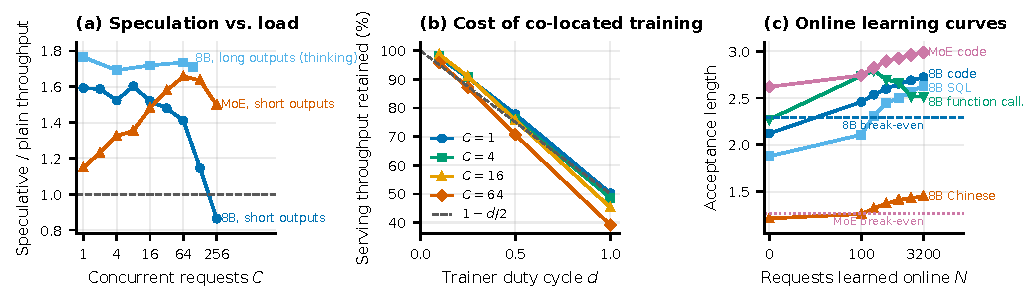
\includegraphics[width=\linewidth]{figures/fig1_motivation.pdf}
\caption{Calibration measurements (one H100, vLLM 0.27.1, factory EAGLE-3 drafters, $k{=}3$). (a) Speculative over plain-decoding throughput versus concurrency. (b) Serving throughput retained when a trainer shares the GPU at duty cycle $d$ (Qwen3-8B, short outputs, speculation on); the dashed line is $1-d/2$. (c) Acceptance length after learning online from $N$ requests; dashed lines mark the break-even acceptance at $C{=}256$ (Qwen3-8B code: \nv{astar.code.c256}; MoE code: \nv{astar.moe.c256}).}
\label{fig:motivation}
\end{figure*}


\section{Related Work}\label{sec:related}

\paragraph{Runtime control of speculative decoding.}
Speculative decoding accelerates autoregressive generation by verifying draft tokens in parallel while preserving the target model's output distribution \citep{leviathan2023fast,chen2023accelerating,miao2024specinfer}. Draft architectures such as Medusa and EAGLE-3 improve the efficiency of token proposals \citep{cai2024medusa,li2024eagle,li2024eagle2,li2025eagle3}. Beyond draft quality, serving performance depends on when and how speculation is used. TurboSpec \citep{liu2024turbospec} selects a speculation length, including zero, based on estimated goodput; AdaSpec \citep{huang2025adaspec} accounts for latency SLOs; Nightjar \citep{li2025nightjar} disables unprofitable speculation and offloads the drafter; and FASER \citep{chen2026faser} adjusts speculation length per request. MoESD \citep{huang2025moesd} and MagicDec \citep{sadhukhan2025magicdec} further show that the profitability of speculation depends on target architecture, batch size, and sequence length. These methods optimize speculative execution given a drafter. Our setting adds a second decision: whether spending resources to improve that drafter will increase future serving throughput enough to justify the cost.

\paragraph{Online drafter adaptation.}
Online speculative decoding addresses draft--target mismatch by updating the drafter from serving traffic. OSD \citep{liu2024osd} uses online distillation to adapt to changing query distributions, while OnlineSPEC \citep{qian2026drafts} develops online-learning algorithms with dynamic-regret guarantees. DVI \citep{bhansali2025dvi} learns from acceptance and rejection signals, and related work explores online drafter selection \citep{liu2026notabandit} and co-training during reinforcement-learning rollouts \citep{wang2026cotraining}. These approaches primarily improve how a drafter learns from available feedback. Our controller treats the learning process itself as a serving decision: higher acceptance is useful only when the resulting throughput gain justifies the resources consumed by adaptation.

\paragraph{Joint training and serving: Aurora and TIDE.}
Aurora \citep{wang2026aurora} closes the training--serving loop through asynchronous reinforcement learning from live inference traces, using a separate training server and hot-swapping updated drafters into serving. Its emphasis is on rapid adaptation, feedback efficiency, and deployment without extensive offline draft training. TIDE \citep{park2026tide} goes further in runtime coordination: it reuses target-model hidden states for training, enables speculation according to batch-dependent profitability, and selectively resumes training when acceptance drifts, retaining updates that improve acceptance. Its deployment separates inference and training across GPU resources, including heterogeneous accelerators. Both systems demonstrate that drafter training and speculative serving can operate together, and TIDE already controls when to speculate and when to adapt. Our work addresses a different resource constraint. Training shares the serving GPU, so each update directly reduces the capacity available to process requests. We therefore estimate not only whether speculation is profitable at the current load, but also whether further adaptation can improve serving enough to repay its interference cost over the expected workload duration. Per-domain learning estimates help identify cases where improvement is insufficient, while the payback calculation limits training even when the drafter can continue to improve.

\paragraph{Co-located training and inference.}
Resource sharing between training and inference has also been studied outside speculative decoding. FlexLLM \citep{oliaro2024flexllm} co-schedules inference with fine-tuning workloads under latency constraints. Our setting differs because training changes the model used by the serving process itself: allocating more GPU time to training immediately reduces serving capacity but may improve subsequent speculative decoding. The controller makes this trade-off explicitly, allocating training from available slack under light load and evaluating its expected net benefit under saturation.

\section{Method}\label{sec:method}

\paragraph{Setting and objective.} One GPU serves a target model with an EAGLE-3 drafter and also runs a trainer that updates a copy of the drafter from features exported during serving (\cref{sec:system}). The drafter proposes $k{=}3$ tokens per step and the target verifies them in one forward pass, so the acceptance length $a$, the number of tokens emitted per verification step, lies between 1 and 4. Every second the controller reads the number of running requests $C$, whether requests are queued, the acceptance length (smoothed by an exponential moving average, $\hat a$), and the trainer's progress. An operator-provided label $\ell$ names the current traffic domain, for example a product line; a \emph{regime} is a period with one label. The controller sets whether speculation is enabled ($z\in\{0,1\}$), the trainer's duty cycle $d\in\mathcal D=\{0,0.1,0.25,0.5,1\}$, and when the trainer exports a drafter, which is then hot-swapped into the server. Its objective is the output throughput served over the regime under an SLO that bounds the time per output token (TPOT) by twice the single-request decode time, $\Tslo$ (\nv{slo.m1}\,ms for Qwen3-8B, \nv{slo.m2}\,ms for the MoE target); it pursues this objective one second at a time, from the predictions below. Figure~\ref{fig:controller} summarizes the loop.

\paragraph{Profitability frontier.} At concurrency $C$, speculation pays when its throughput exceeds that of plain decoding, i.e., when the ratio $G(a,C)$ of the two exceeds one. Verification makes every step more expensive, and at high concurrency the GPU has no spare compute to absorb this cost, so the break-even acceptance $a^{*}(C)$ at which $G=1$ rises with load. The ratio is close to linear in acceptance at every load (\cref{sec:measure}), so for each domain $\ell$ we fit, from the throughput of a few drafter checkpoints at a few loads,
\begin{equation}
\Ghat_\ell(a,C)=\alpha_\ell(C)\,a+\beta_\ell(C),\qquad a^{*}_\ell(C)=\frac{1-\beta_\ell(C)}{\alpha_\ell(C)}.\label{eq:frontier}
\end{equation}
As the drafter trains, its operating point moves along the acceptance axis of this frontier.

\paragraph{Calibration.} Before deployment we measure, once per target, the plain and speculative step times and plain throughput as functions of $C$, the interference coefficient $\kappa(C)$ (serving throughput falls by $\kappa(C)\,d$ at duty $d$), and the trainer's token rate $r$ at full duty; and once per domain, the frontier of \cref{eq:frontier} and the learning curve $a_\ell(N)$, the acceptance after learning from $N$ requests (\cref{sec:measure,app:calibration}). From these the controller predicts the throughput $\Theta(a,z,C)$ and the TPOT for any acceptance, speculation state, and duty (\cref{app:controller}). It never trains on a domain without a learning curve.

\paragraph{When to speculate.} Speculation is enabled when the current drafter beats plain decoding at the current load,
\begin{equation}
z=\mathbf{1}\big[\Ghat_\ell(\hat a,C)>1\big]\wedge\big(\widehat T_{\mathrm{spec}}\le\Tslo\vee\widehat T_{\mathrm{plain}}>\Tslo\big),\label{eq:switch}
\end{equation}
where the second clause keeps plain decoding if speculation would push an otherwise compliant load out of the SLO. A switch needs three agreeing ticks and happens at most once per 10\,s; since acceptance cannot be measured with speculation off, every drafter swap is followed by an 8\,s probe with speculation on.

\paragraph{Whether training can pay at all.} Let $\amax_\ell=\max_N a_\ell(N)$ be the domain's ceiling. If even the ceiling loses to plain decoding at the current load, $\Ghat_\ell(\amax_\ell,C)\le1$, no amount of training makes speculation worthwhile: the controller does not train, and \cref{eq:switch} turns speculation off instead (the \emph{structural-ceiling} test). Training also stops when the drafter is within 0.02 of its ceiling, or when the last swapped drafter raised the measured acceptance by less than 0.02.

\paragraph{How much to train.} If the predicted TPOT is within the SLO and no request is queued, the GPU has spare capacity and training costs latency but no throughput. The controller then picks the largest $d\in\mathcal D$ whose predicted TPOT stays below $0.9\,\Tslo$, i.e., $T_0/(1-\kappa(C)\,d)\le0.9\,\Tslo$, where $T_0$ is the predicted TPOT without training. Under saturation (requests queued, or $C$ at 95\% of the batch limit), training costs throughput immediately. The controller sets a target acceptance $a^{\dagger}=\hat a+0.8\,(\amax_\ell-\hat a)$, reads from the learning curve how many training tokens $n$ separate $\hat a$ from $a^{\dagger}$, and scores each $d\le0.5$ by
\begin{equation}
\begin{aligned}
V(d)={}&\big[\Theta^{\star}(a^{\dagger})-\Theta(\hat a)\big]\,\max\!\big(0,\widehat H-\tau(d)\big)\\
&-\Theta(\hat a)\,\kappa(C)\,b(d)\,\tau(d).
\end{aligned}\label{eq:value}
\end{equation}
Here $\tau(d)=n/\min(rd,\rho)$ is the training time when training data become available at rate $\rho$, $b(d)=\min(d,\rho/r)$ is the trainer's actual busy fraction, $\Theta^{\star}$ is the better of speculation on and off, and $\widehat H$ is the forecast remaining length of the regime. The first term is the gain once the improved drafter is in place, the second the loss while it trains. The controller trains at $\arg\max_d V(d)$ if the maximum is positive and not at all otherwise. Not knowing when the regime will end, it forecasts $\widehat H$ as the regime's age so far, clipped to $[90,600]$\,s.

\paragraph{Export and swap.} The trainer exports a drafter after 100, 200, 400, \dots{} requests learned in the current regime, and each export is swapped in immediately. When the label changes, the trainer's buffer is flushed and the schedule restarts.

\paragraph{What the controller assumes.} It needs the label and a per-domain calibration from a short profiling run, but neither the regime's end nor the right time to stop; its rules and constants (\cref{app:controller}) were fixed before the evaluation checkpoint was frozen and not changed afterwards.

\begin{figure*}[t]
\centering
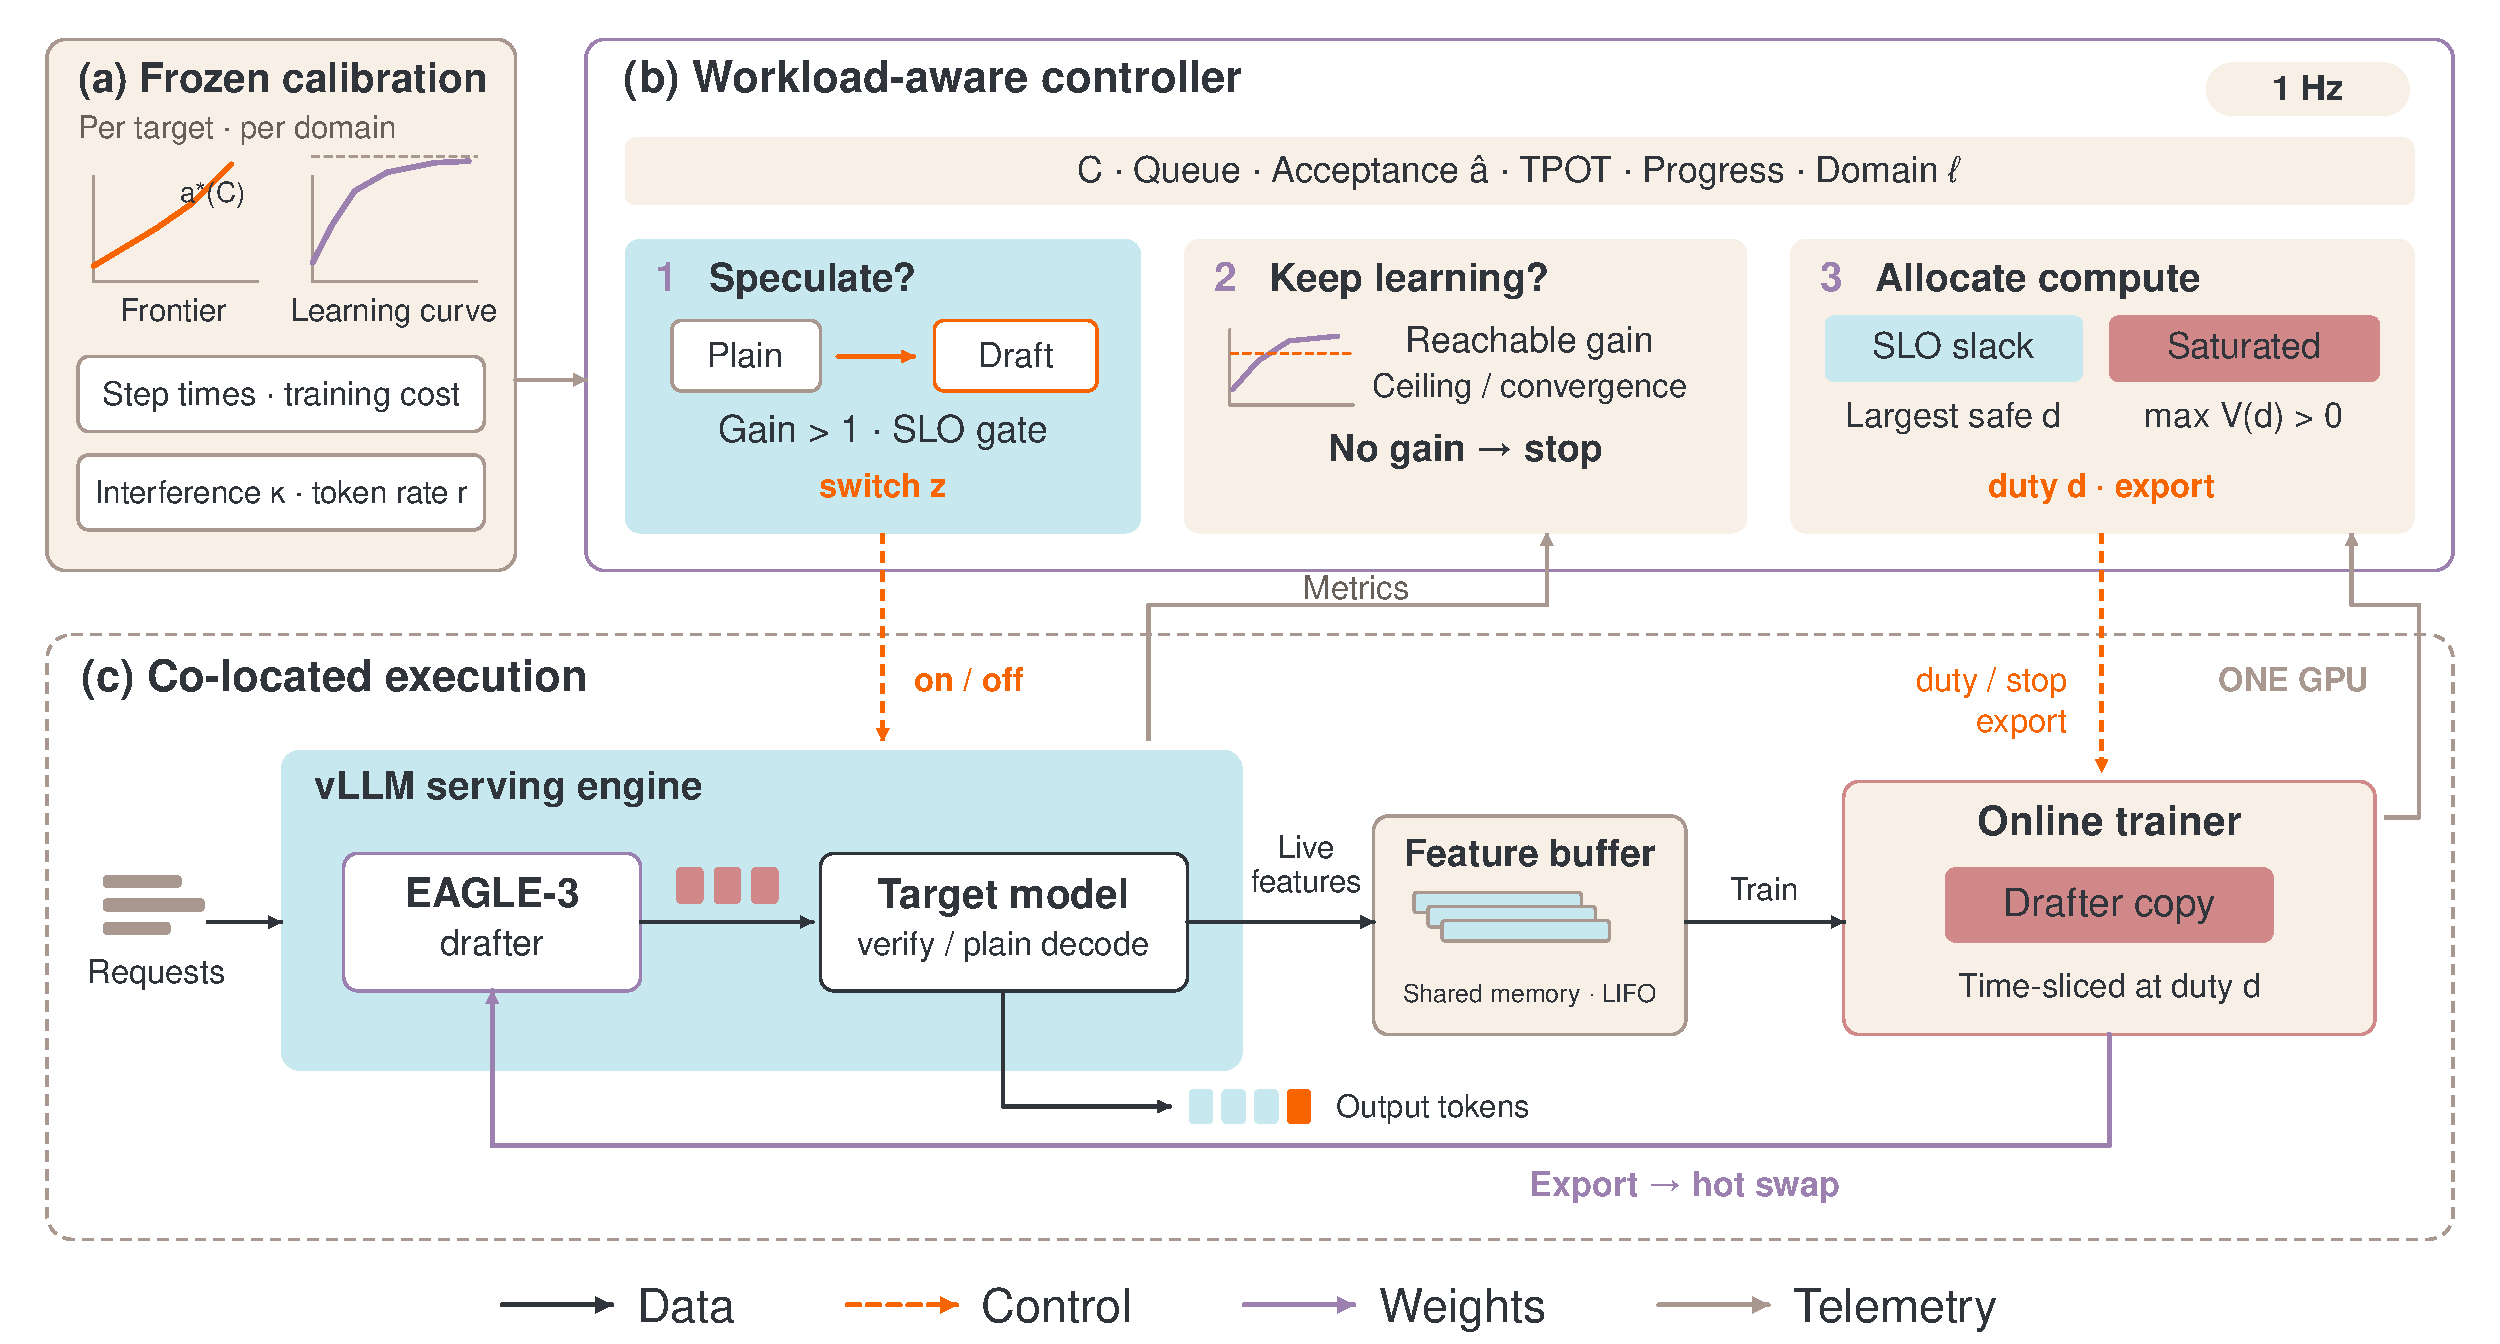
\includegraphics[width=\linewidth]{figures/fig2.pdf}
\captionsetup{skip=2pt}
\caption{The control loop. Each second the controller combines engine and trainer measurements with the frozen calibration and applies three tests: whether the current drafter beats plain decoding (\cref{eq:switch}), whether training can still pay (structural ceiling, ceiling, convergence), and how much to train (SLO slack, or the value of \cref{eq:value} under saturation). Its outputs are a speculation switch, the trainer's duty cycle, and drafter exports that are hot-swapped into the running engine.}
\label{fig:controller}
\end{figure*}

\section{System and Experimental Setup}\label{sec:system}

\subsection{Implementation in vLLM}\label{sec:impl}

We implement the system on vLLM 0.27.1 (V1 engine) with three engine extensions and two processes beside the server.

\paragraph{Live feature export.} The trainer needs the target's auxiliary hidden states at every accepted position. Inside the EAGLE-3 path of the model runner, we copy them from the GPU to pinned host memory without blocking the step, and a background thread writes them per request into a shared-memory ring buffer. Rejected positions are dropped, only tensor-parallel rank 0 writes, and a full buffer drops one step instead of stalling serving. Prefix caching has to be disabled, because positions served from the cache have no hidden states.

\paragraph{Co-located trainer.} A separate process on the same GPU trains the drafter with cross-entropy against the target's own next tokens over the drafter's vocabulary (AdamW; \cref{app:manifest}). It reads completed requests from the ring buffer into a last-in-first-out buffer of at most 600k tokens, discards data older than 60\,s, and implements duty cycle $d$ by sleeping $(1-d)/d$ times the duration of each step.

\paragraph{Drafter hot swap and speculation switch.} A collective RPC loads new drafter weights into all workers without restarting the engine; in the frozen runs a swap took a median of \nv{swap.m1.med}\,s for the Qwen3-8B drafter and \nv{swap.m2.med}\,s for the MoE drafter. A second RPC switches speculation in the scheduler and the workers together, so drafting stops instead of being computed and discarded; the drafter stays in GPU memory and the round trip takes a median of \nv{switch.med}\,ms.

\paragraph{Controller process.} The controller is a 1\,Hz process that reads the engine's metrics endpoint and the trainer's log, writes the duty cycle to a file that the trainer reads before every step, and requests exports through a command file.

\subsection{Experimental protocol}\label{sec:setup}

\paragraph{One frozen checkpoint.} Every experiment runs on one checkpoint that we froze before the first run: the controller, trainer, and harness code, the six patched engine files, the two calibration files, the factory drafters, the target weights, the prompt pools, the seeds, and the software environment, each recorded by hash (\cref{app:manifest}). \pol{TIDE} was added later as new files only and, like the reruns below, runs in an environment rebuilt from the frozen package list.

\paragraph{Workload.} Each run serves three phases on one H100 GPU: 200 chat requests at concurrency 16 (phase A1), then 16{,}000 unique requests from a new domain at concurrency 256, which saturate the GPU for \nv{bdur.min}--\nv{bdur.max}\,s (phase B), then 200 different chat requests (phase A2). The scenarios are Qwen3-8B with code or Chinese in B and Qwen3-30B-A3B with code in B. Decoding is greedy, outputs stop naturally or at 512 tokens, and the B prompts were never seen during calibration. All policies except \pol{Production} reserve the trainer's memory (\cref{app:manifest}).

\paragraph{Policies.} \pol{Production} runs the factory drafter with speculation always on, without export or memory reserve, as deployed today. \pol{Static} does the same under the evaluation's engine configuration and is the reference for all differences. \pol{Plain} serves without a drafter. \pol{Switch} applies \cref{eq:switch} with the domain's frontier and never trains. \pol{Threshold} turns speculation off whenever the server is saturated and trains at duty 0.5 whenever the predicted TPOT is within the SLO, i.e., the idle-time rule of OSD \citep{liu2024osd} combined with a load threshold. \pol{TIDE} reimplements the training triggers of TIDE \citep{park2026tide} with the speculation rule of \pol{Switch}: it trains at duty 0.5 from the start and whenever acceptance drifts down, swaps in a drafter every 200 requests learned, and restores the previous one and stops if acceptance did not rise. \pol{Always} trains at duty 0.5 from the first request and swaps drafters after 100, 200, 400, \dots{} requests. \pol{Informed} trains at duty 0.5 from the moment phase B starts until it has learned from 800 requests, swapping at 100, 200, 400, and 800; its stopping point comes from the learning curves of \cref{fig:motivation}c, so it is a reference that knows when to stop, not a deployable policy. \pol{Full} is the controller of \cref{sec:method}. Neither turns speculation off (\cref{app:policies}).

\paragraph{Repetitions and metrics.} Every policy runs three times per scenario. Repetition $r$ fixes the prompt order of all phases and the trainer's random seed, so within a repetition all policies serve the same request sequence, and we report paired differences as mean $\pm$ standard deviation over the three pairs. The main metric is phase-B output throughput; we also report TPOT and whole-run throughput. The \nv{n.runs} runs used \nv{hosts} nodes of the same type and \nv{gpuh} GPU-hours. A scan with a rule fixed in advance found node interference in \nv{scan.flagged.word} of the \nv{scan.n} runs, all of them baselines; we report their reruns, which can only narrow the controller's margins (\cref{app:rerun}).

\paragraph{Further conditions.} Four ablations remove one of \pol{Full}'s tests at a time (payback rule, stop tests, speculation switch, or label and learning curve) on the same checkpoint, prompts, and seeds (\cref{app:ablation}). Two mixed-traffic scenarios serve a 50/50 mixture of code or Chinese with chat in phase B, calibrated as domains of their own, with \pol{Full} also run under a stale label and without any label (\cref{app:mix}). Five policies were rerun on a port to SGLang 0.5.10 with its own frozen calibration (\cref{app:sglang}), and a fluid simulator built from the frozen calibration replays unseen traces against four criteria declared before the runs (\cref{app:sim}).

\section{Experimental Results}\label{sec:evaluation}

\subsection{Speculation profitability and training cost}\label{sec:measure}

The calibration measurements (\cref{app:calibration}; Figure~\ref{fig:motivation}) show the three effects that make speculation and training one decision.

\paragraph{Whether speculation pays depends on load and architecture.} For Qwen3-8B with short outputs, speculation is \nv{sweep.short.c1}\% faster than plain decoding at $C{=}1$ but \nv{sweep.short.c256abs}\% slower at $C{=}256$ (Figure~\ref{fig:motivation}a); with long outputs it remains \nv{sweep.long.c96}\% faster at $C{=}96$. The MoE target behaves the other way: its gain grows to \nv{sweep.moe.c64}\% at $C{=}64$ and is still \nv{sweep.moe.c256}\% at $C{=}256$, because a speculative step costs only \nv{step.m2.c256}$\times$ a plain step there, against \nv{step.m1.c256}$\times$ on the dense target \citep{huang2025moesd}.

\paragraph{Co-located training is not free.} At duty cycle $d$ the trainer computes for a fraction $d$ of the time, and serving throughput falls almost linearly, by $\kappa(C)\,d$ with $\kappa$ between \nv{kappa.min} and \nv{kappa.max} (Figure~\ref{fig:motivation}b): duty 0.5 costs \nv{duty.d05.lossmin}--\nv{duty.d05.lossmax}\% of throughput, and training all the time costs \nv{duty.d10.lossmin}--\nv{duty.d10.lossmax}\%.

\paragraph{Learning ceilings differ, and the frontier is linear.} After learning online from $N$ requests (Figure~\ref{fig:motivation}c), the code and SQL drafters improve steadily, the Chinese drafter stalls at \nv{lc.zh.n3200} because only \nv{cover.zh}\% of the target's output tokens are in its 32k draft vocabulary, and the function-calling drafter peaks at $N{=}\nv{lc.fc.peakN}$ and then declines. Against the break-even line at $C{=}256$, the code drafter crosses after about 100 requests, the Chinese drafter never does, and the MoE drafter is above its much lower break-even (\nv{astar.moe.c256}) from the start. The throughput ratio of three or four drafter checkpoints at six loads is close to linear in acceptance at every load (Figure~\ref{fig:frontier}): the fit of \cref{eq:frontier} has residuals of at most \nv{astar.code.err} (code), \nv{astar.zh.err} (Chinese), and \nv{astar.moe.err} (MoE), and the adapted code drafter reaches \nv{fr.code.n3200.c256}$\times$ plain decoding there against \nv{fr.code.n0.c256}$\times$ for the factory drafter. Training is therefore worth doing only if the trained drafter will be used, which depends on load, and at saturation the drafter may become usable only after training.

\subsection{End-to-end serving performance}\label{sec:results}

\begin{table*}[t]
\caption{Phase-B (saturated) throughput relative to \pol{Static}: paired mean $\pm$ sd over three repetitions, \%. Parentheses: fraction of the best policy in the scenario (bold); \pol{Static} row: absolute throughput; last column: smallest fraction over the three scenarios.}
\label{tab:main}
\centering\small

% Generated table style: Main Results
\renewcommand{\arraystretch}{1.15}
\setlength{\tabcolsep}{4pt}

\begin{tabular}{@{}lcccc@{}}
\toprule
\textbf{Policy} &
\textbf{8B Code} &
\textbf{8B Chinese} &
\textbf{MoE Code} &
\textbf{Worst Case} \\
\midrule

% ===== Serving baselines =====
\rowcolor{tabGroup}
\textbf{\footnotesize Serving baselines}
& & & & \\

Production speculation
& $+2.2\pm0.9$\,{\scriptsize(0.854)}
& $+1.8\pm0.8$\,{\scriptsize(0.517)}
& $+1.0\pm0.1$\,{\scriptsize(0.923)}
& 0.517 \\

Static speculation
& 14{,}282 tok/s\,{\scriptsize(0.835)}
& 8{,}526 tok/s\,{\scriptsize(0.508)}
& 13{,}859 tok/s\,{\scriptsize(0.915)}
& 0.508 \\

Plain decoding
& $+18.1\pm0.9$\,{\scriptsize(0.986)}
& \cellcolor{tabBest}
  $\boldsymbol{+97.0\pm1.4}$\,{\scriptsize\bfseries(1.000)}
& $-46.1\pm0.1$\,{\scriptsize(0.493)}
& 0.493 \\

\addlinespace[3pt]

% ===== Reactive runtime policies =====
\rowcolor{tabGroup}
\textbf{\footnotesize Reactive runtime policies}
& & & & \\

Switch only
& $+12.9\pm2.5$\,{\scriptsize(0.943)}
& $+90.9\pm2.2$\,{\scriptsize(0.969)}
& $-0.3\pm0.3$\,{\scriptsize(0.912)}
& 0.912 \\

Threshold rule
& $+14.8\pm0.8$\,{\scriptsize(0.959)}
& $+86.9\pm4.7$\,{\scriptsize(0.949)}
& $-46.0\pm0.0$\,{\scriptsize(0.494)}
& 0.494 \\

TIDE-style triggers
& $+13.8\pm3.5$\,{\scriptsize(0.950)}
& $+54.5\pm3.6$\,{\scriptsize(0.784)}
& $+6.0\pm4.0$\,{\scriptsize(0.970)}
& 0.784 \\

\addlinespace[3pt]

% ===== Fixed training schedules =====
\rowcolor{tabGroup}
\textbf{\footnotesize Training schedules}
& & & & \\

Always train
& $+2.4\pm1.9$\,{\scriptsize(0.855)}
& $-1.2\pm0.7$\,{\scriptsize(0.502)}
& $-3.6\pm0.3$\,{\scriptsize(0.882)}
& 0.502 \\

\cellcolor{tabOracle}Informed schedule
& \cellcolor{tabBest}
  $\boldsymbol{+19.7\pm0.5}$\,{\scriptsize\bfseries(1.000)}
& $+13.8\pm0.4$\,{\scriptsize(0.578)}
& \cellcolor{tabBest}
  $\boldsymbol{+9.3\pm0.7}$\,{\scriptsize\bfseries(1.000)}
& 0.578 \\

\addlinespace[3pt]

% ===== Proposed controller =====
\rowcolor{tabGroup}
\textbf{\footnotesize Proposed method}
& & & & \\

\rowcolor{tabFull}
\textbf{Full controller}
& $+18.0\pm1.6$\,{\scriptsize(0.985)}
& $+87.7\pm8.5$\,{\scriptsize(0.953)}
& $+8.0\pm0.4$\,{\scriptsize(0.988)}
& \cellcolor{tabBest}\textbf{0.953} \\

\bottomrule
\end{tabular}

\end{table*}

Table~\ref{tab:main} shows the frozen matrix (per-repetition values in Figure~\ref{fig:policies}, \cref{app:extra}). The best policy is \pol{Plain} for Qwen3-8B Chinese and \pol{Informed} for both code scenarios, and every policy other than \pol{Full} falls well short in at least one scenario. \pol{Plain} and \pol{Threshold} lose about half of the MoE throughput, because they turn speculation off where it is still \nv{fr.moe.n0.c256}$\times$ faster than plain decoding. \pol{Informed} keeps speculating on Chinese and reaches only \nv{zh.informed.r} of \pol{Plain}; \pol{TIDE} keeps training there and reaches \nv{zh.tide.r}. \pol{Switch}, which never trains, is the most robust alternative but still falls \nv{switch.worstshort}\% short on MoE. \pol{Full} is the only policy within 5\% of the best in every scenario (worst case \nv{full.worst}). Against \pol{Static} it raises phase-B throughput by \nv{code.full.d}$\pm$\nv{code.full.sd}\%, \nv{zh.full.d}$\pm$\nv{zh.full.sd}\%, and \nv{moe.full.d}$\pm$\nv{moe.full.sd}\%, with the same sign in every repetition (\nv{code.full.session}\%, \nv{zh.full.session}\%, and \nv{moe.full.session}\% over \pol{Production} for the whole run).

\paragraph{Against the informed schedule.} Relative to \pol{Informed}, \pol{Full} is \nv{code.full_vs_informed}\% on Qwen3-8B code, within the run-to-run spread, and \nv{moe.full_vs_informed}\% on MoE, with the same sign in all three repetitions. \pol{Always}, which never stops training, ends close to \pol{Static} (\nv{code.always.d}\%, \nv{zh.always.d}\%, \nv{moe.always.d}\%): continuous training costs as much throughput as the better drafter gains. We therefore do not claim that the controller beats a well-chosen fixed schedule where one exists; it matches such schedules within 1.5\% without knowing when to stop, and it does not fail where they do.

\subsection{Decision analysis and ablations}\label{sec:levers}

\begin{table*}[t]
\caption{What \pol{Full} did in phase B (means over three runs): share of time with speculation on, mean duty, drafter swaps, acceptance at the start and end of B, tokens trained in the run, and the training tests' decisions as a share of ticks (below 5\% omitted).}
\label{tab:behaviour}
\centering\small

% Controller behavior during the saturated phase
\begingroup
\renewcommand{\arraystretch}{1.18}
\setlength{\tabcolsep}{3.5pt}

\begin{tabularx}{\linewidth}{@{}
    lccccc>{\raggedright\arraybackslash}X@{}}
\toprule
\textbf{Scenario} &
\textbf{Spec.\ on} &
\textbf{Duty} &
\textbf{Swaps} &
\textbf{Acceptance} &
\shortstack{\textbf{Train tok.}\\\textbf{(M)}} &
\textbf{Decisions during saturation (share of 1\,s ticks)} \\
\midrule

% ===== Dense target =====
\rowcolor{tabGroup}
\multicolumn{7}{@{}l}{
    \textbf{Qwen3-8B (Dense)}
} \\

8B code
& \textbf{100\%}
& 0.067
& 3
& \cellcolor{tabFull}
  $\boldsymbol{2.50\rightarrow2.66}$
& 0.64
& No training (value $\leq 0$) \textbf{77\%};
  train (value $>0$) 10\%;
  converged 10\% \\

8B Chinese
& \textbf{2\%}
& 0.016
& 1
& $1.18\rightarrow1.18$
& 0.38
& \cellcolor{tabFull}
  \textbf{Structural ceiling 97\%} \\

\addlinespace[3pt]

% ===== Mixture-of-experts target =====
\rowcolor{tabGroup}
\multicolumn{7}{@{}l}{
    \textbf{Qwen3-30B-A3B (MoE)}
} \\

MoE code
& \textbf{100\%}
& 0.084
& 4
& \cellcolor{tabFull}
  $\boldsymbol{2.68\rightarrow2.97}$
& 0.81
& At ceiling \textbf{43\%};
  no training (value $\leq 0$) 36\%;
  train (value $>0$) 19\% \\

\bottomrule
\end{tabularx}
\endgroup

\end{table*}

\begin{table}[t]
\caption{Phase-B throughput of \pol{Full} with one test removed, relative to \pol{Full} (paired mean $\pm$ sd over three repetitions, \%).}
\label{tab:ablate}
\centering\small\setlength{\tabcolsep}{4pt}
\IfFileExists{tables/tab_ablate_main.tex}{
% Ablation study: effect of removing individual tests
\begingroup
\renewcommand{\arraystretch}{1.20}
\setlength{\tabcolsep}{5pt}

\begin{tabular}{@{}lccc@{}}
\toprule
\textbf{Variant of \pol{Full}} &
\textbf{8B Code} &
\textbf{8B Chinese} &
\textbf{MoE Code} \\
\midrule

% ===== Training-control decisions =====
\rowcolor{tabGroup}
No payback rule
& $-2.5\pm2.6$
& $+2.4\pm4.2$
& $+0.4\pm1.7$ \\

\rowcolor{tabGroup}
No stop tests
& $-0.2\pm1.1$
& $+1.8\pm2.5$
& $-0.9\pm0.3$ \\

\addlinespace[3pt]

% ===== Speculation-control decision =====
No speculation switch
& $+0.2\pm1.6$
& \cellcolor{tabDrop}
  $\boldsymbol{-43.8\pm2.2}$
& $+0.1\pm0.6$ \\

\addlinespace[3pt]

% ===== Calibration dependence =====
No label or curve
& $-0.6\pm2.7$
& $-0.1\pm6.6$
& $-0.9\pm1.5$ \\

\bottomrule
\end{tabular}
\endgroup
}{}
\end{table}

\paragraph{Chinese: turn speculation off.} The controller acts differently in the three scenarios (\cref{tab:behaviour}). On Chinese the structural-ceiling test decides \nv{zh.full.why.structural_ceiling}\% of the ticks: even the best reachable drafter (\nv{lc.zh.n3200}) is below break-even at this load, so the controller keeps speculation off except for short probes and spends almost no time training (mean duty \nv{zh.full.duty}). It ends \nv{zh.full_vs_plain}\% from \pol{Plain}, the cost of the engine's speculation-off state (\pol{Switch}: \nv{zh.switch_vs_plain}\%; \cref{sec:overheads}).

\paragraph{Qwen3-8B code: adapt and keep speculating.} The controller never turns speculation off. It enters phase B with acceptance \nv{code.full.acc0} instead of the factory \nv{code.static.acc0}, because it already trained in the SLO slack of phase A1 and the chat-trained drafter transfers to code; during B it trains at a mean duty of \nv{code.full.duty}, swaps \nv{code.full.swaps} drafters, reaches \nv{code.full.acc1}, and the value rule declines to train in \nv{code.full.why.saturated_no_value}\% of the ticks. The adapted drafter makes speculation as fast as plain decoding at $C{=}256$ (\nv{code.full_vs_plain}\%), which is \nv{code.full_vs_switch}$\pm$\nv{code.full_vs_switch.sd}\% relative to \pol{Switch}, about what the engine's speculation-off state costs.

\paragraph{MoE code: adaptation is the whole gain.} Turning speculation off would halve throughput, and the controller keeps it on; it trains at a mean duty of \nv{moe.full.duty}, swaps \nv{moe.full.swaps} drafters, raises acceptance from \nv{moe.full.acc0} to \nv{moe.full.acc1}, and stops at the ceiling (\nv{moe.full.why.at_ceiling}\% of ticks). Relative to \pol{Switch} it is \nv{moe.full_vs_switch}$\pm$\nv{moe.full_vs_switch.sd}\%, while \pol{Threshold}, which turns speculation off, loses \nv{moe.thresh.abs}\%.

\paragraph{Why acceptance-triggered training falls short.} \pol{TIDE} speculates by the same frontier but trains when observed acceptance suggests it (\cref{tab:tide}). On Chinese it trains for \nv{zh.tide.trainB}\% of phase B, because acceptance is measured only while speculation is on, so its drift trigger keeps restarting training (within two seconds of \nv{zh.tide.rejdrift} of its \nv{zh.tide.rej} rejections) for drafters that never reach break-even; \pol{Full} is \nv{zh.full_vs_tide}\% relative to it. On code it stops after the first round that does not raise acceptance: beyond 400 requests a round of 200 adds at most \nv{tide.roundgain.max}, within the $\pm$\nv{tide.noise.m2} spread of its 8\,s comparison, whereas doubling export gaps keep later gains measurable; \pol{Full} is \nv{code.full_vs_tide}\% relative to it on Qwen3-8B code, positive in every repetition, and \nv{moe.full_vs_tide}\% on MoE, within the spread, also with larger rounds and a larger drift margin (\cref{app:tidevar}).

\paragraph{Which test the gain comes from.} \Cref{tab:ablate} removes one test at a time (\cref{app:ablation}). The gain comes from a different test in each scenario. On Chinese it comes entirely from the switch: without it the controller is \nv{abl.noswitch.zh.vsv6}\% below \pol{Full} (\nv{abl.noswitch.zh.min} to \nv{abl.noswitch.zh.max}\% per repetition), while the other three variants stay within noise. On Qwen3-8B code it comes from training, and the payback rule is worth \nv{abl.novalue.code.vsv6.abs}\%: at a fixed duty the trainer runs until the ceiling test stops it (mean duty \nv{abl.novalue.code.duty} against \nv{code.full.duty}), and the interference costs more than the last drafters gain. On the MoE target every variant trains and stops at the ceiling. The stop tests add nothing under saturation (\nv{abl.nostop.code.vsv6}\%, \nv{abl.nostop.zh.vsv6}\%, \nv{abl.nostop.moe.vsv6}\%), because near the ceiling the payback rule already finds no value. The variant without labels or learning curves stays within noise of \pol{Full} in all three scenarios (\nv{abl.nocurve.code.vsv6}\%, \nv{abl.nocurve.zh.vsv6}\%, \nv{abl.nocurve.moe.vsv6}\%): the switch needs only the measured acceptance and the per-target step times, and the measured swap gains replace the learning curve.

\subsection{Robustness to mixed and unseen workloads}\label{sec:robust}

\begin{table}[t]
\caption{Mixed traffic (Qwen3-8B; phase B a 50/50 mixture): phase-B throughput relative to \pol{Static} (paired mean $\pm$ sd, \%; ratio to the best policy in parentheses).}
\label{tab:mix}
\centering\footnotesize\setlength{\tabcolsep}{4pt}
\IfFileExists{tables/app_mix.tex}{
% Mixed-traffic results -- grouped by model and policy type
\begingroup
\renewcommand{\arraystretch}{1.20}
\setlength{\tabcolsep}{5pt}

\begin{tabular}{@{}lcc@{}}
\toprule

% ===== Model group =====
&
\multicolumn{2}{c}{
  \textbf{Qwen3-8B (Dense)}
} \\
\cmidrule(l){2-3}

\textbf{Policy}
& \textbf{Code + Chat}
& \textbf{Chinese + Chat} \\
\midrule

% ===== Baseline policies =====
\rowcolor{tabGroup}
\multicolumn{3}{@{}l}{
  \textbf{\footnotesize Baseline Policies}
} \\

Static
& 12{,}748 tok/s\,{\scriptsize(0.822)}
& 10{,}138 tok/s\,{\scriptsize(0.650)} \\

Plain
& \cellcolor{tabBest}
  $\boldsymbol{+21.7\pm0.6}$\,
  {\scriptsize\bfseries(1.000)}
& \cellcolor{tabBest}
  $\boldsymbol{+53.7\pm0.4}$\,
  {\scriptsize\bfseries(1.000)} \\

Switch
& $+19.3\pm0.4$\,{\scriptsize(0.980)}
& $+50.0\pm0.7$\,{\scriptsize(0.976)} \\

TIDE
& $+16.9\pm0.5$\,{\scriptsize(0.961)}
& $+44.8\pm2.9$\,{\scriptsize(0.942)} \\

\addlinespace[3pt]

% ===== Proposed controller and variants =====
\rowcolor{tabGroup}
\multicolumn{3}{@{}l}{
  \textbf{\footnotesize Proposed Controller and Variants}
} \\

\rowcolor{tabFull}
\textbf{Full}
& $+16.0\pm2.1$\,{\scriptsize(0.953)}
& $+50.4\pm0.3$\,{\scriptsize(0.978)} \\

Full, stale label
& $+14.7\pm0.5$\,{\scriptsize(0.942)}
& $+48.3\pm0.4$\,{\scriptsize(0.965)} \\

Full, label-free
& $+13.0\pm3.6$\,{\scriptsize(0.928)}
& $+50.0\pm1.0$\,{\scriptsize(0.976)} \\

\bottomrule
\end{tabular}
\endgroup
}{}
\end{table}

\paragraph{Mixed traffic and stale labels.} Production traffic is often a mixture without a clean switch point, and the label can be stale. \Cref{tab:mix} serves 50/50 mixtures of code or Chinese with chat (\nv{mix.n.runs} runs; \cref{app:mix}). Neither pays for speculation at saturation, so \pol{Plain} is best and the others rank by how little they lose. Chinese--chat has a structural ceiling: \pol{Full} turns speculation off on the first tick and does not train, within noise of \pol{Switch} (\nv{mix.zc.v6.vsswitch}\%); the label-free variant reaches the same decision (\nv{mix.zc.v6_nocurve.vsv6}\%), and a stale label costs one wasted training round (\nv{mix.zc.v6_stale.vsv6.abs}\%). Code--chat sits at break-even, where what training can return is within the calibration error: \pol{Full} ends \nv{mix.cc.v6.vsswitch}\% behind \pol{Switch}, and the label-free variant, which trains until measured swap gains stop it, loses \nv{mix.cc.v6_nocurve.vsv6.abs}\% more. The curve is thus worth a few percent only at break-even; a drifting mixture is not covered.

\begin{figure*}[t]
\centering
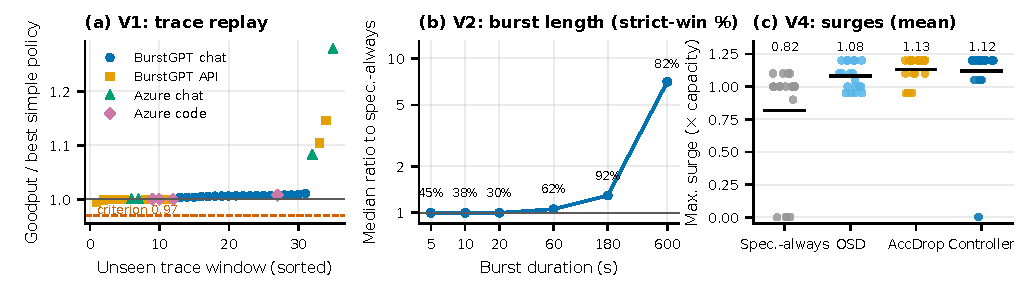
\includegraphics[width=0.58\linewidth]{figures/fig5_heldout.pdf}
\caption{Frozen-simulator validation on unseen workloads: (a) controller goodput relative to the best of five simple policies in each of \nv{v1.n} trace windows (sorted); (b) median goodput relative to \pol{SpecAlways} for bursts of a new domain, by length (labels: share of strict wins); (c) largest surge, in multiples of plain-decoding capacity, served without SLO violation in 20 scenarios (dots) and their mean (bars).}
\label{fig:heldout}
\end{figure*}

\paragraph{Unseen traffic shapes in a frozen simulator.}\label{sec:heldout} To test traffic shapes beyond the live runs, we replay traces in a fluid single-GPU simulator built from the frozen calibration file, with goodput (tokens served within the SLO) as the currency and five simple policies (\pol{NoSpec}, \pol{SpecAlways}, and \pol{OSD}, \pol{Timed}, and \pol{AccDrop}, which train on idle time, a timer, or an acceptance drop). We froze the simulator and the calibration and declared four criteria before running workloads never used in development: \nv{v1.n} unseen trace windows from BurstGPT \citep{wang2024burstgpt} and the Azure 2023 traces \citep{patel2024splitwise} at three or four load scales, 60 random bursts of a new domain, 40 Chinese regimes, and 20 surge scenarios at seven surge levels (\cref{app:sim}).

Figure~\ref{fig:heldout} reports the outcomes (\cref{tab:heldout} in \cref{app:sim}). The goodput criterion holds in all \nv{v1.n} trace windows: the controller is never more than \nv{v1.short}\% below the best simple policy and is the best policy in \nv{v1.best}. The training criterion fails in four Azure chat windows (\pol{OSD} trains on fewer tokens). Three pre-declared expectations did not survive (\cref{app:sim}): training pays back reliably only for bursts of about three minutes or longer (strict wins \nv{v2.d60.win}\% at 60\,s, \nv{v2.d180.win}\% at 180\,s), the controller's margin over \pol{SpecAlways} in the \nv{v3.n} Chinese regimes is \nv{v3.feas.min}--\nv{v3.feas.max}$\times$ rather than the pre-declared $1.5\times$, and \pol{AccDrop} tolerates surges as well as the controller; the controller's advantage lies in meeting all four criteria at once.

\subsection{Cross-engine deployment and runtime overheads}\label{sec:sglang}

\begin{table}[t]
\caption{SGLang: phase-B throughput relative to \pol{Static} (paired mean $\pm$ sd, \%; best in bold) and the worst ratio to the scenario's best policy.}
\label{tab:sgl_main}
\centering\footnotesize\setlength{\tabcolsep}{3pt}
\IfFileExists{tables/tab_sgl_main.tex}{
% SGLang results -- grouped by model architecture
\begingroup
\renewcommand{\arraystretch}{1.20}
\setlength{\tabcolsep}{3pt}

\begin{tabular}{@{}lcccc@{}}
\toprule

% ===== Model architecture groups =====
&
\multicolumn{2}{c}{
  \textbf{Qwen3-8B (Dense)}
}
&
\multicolumn{1}{c}{
  \shortstack{
    \textbf{30B-A3B}
    \textbf{(MoE)}
  }
}
& \\

\cmidrule(lr){2-3}
\cmidrule(lr){4-4}

\textbf{Policy}
& \textbf{Code}
& \textbf{Chinese}
& \textbf{Code}
& \textbf{Worst} \\

\midrule

\pol{Static}
& 10.4k tok/s
& 6.4k tok/s
& 6.8k tok/s
& 0.523 \\

\pol{Plain}
& \cellcolor{tabBest}
  $\boldsymbol{+16.0\pm0.6}$
& \cellcolor{tabBest}
  $\boldsymbol{+91.4\pm0.9}$
& $-31.9\pm0.5$
& 0.628 \\

\pol{Switch}
& $-0.5\pm0.2$
& $+37.9\pm3.9$
& $-0.7\pm0.9$
& \cellcolor{tabBest}\textbf{0.721} \\

\pol{TIDE}
& $+15.8\pm1.0$
& $+35.8\pm1.6$
& \cellcolor{tabBest}
  $\boldsymbol{+8.4\pm1.0}$
& 0.710 \\

\addlinespace[3pt]

% ===== Proposed controller =====
\rowcolor{tabFull}
\pol{Full}
& $+15.8\pm1.0$
& $+37.0\pm6.6$
& $+7.7\pm0.5$
& 0.716 \\

\bottomrule
\end{tabular}
\endgroup
}{}
\end{table}

\paragraph{A second engine.} We reimplemented the three engine extensions on SGLang 0.5.10 \citep{zheng2024sglang} as a runtime patch of its EAGLE-3 path, writing the same shared-memory records, so that the harness, controller, trainer, prompts, and seeds of the vLLM checkpoint run unchanged (\cref{app:sglang}). The port passes its checks: greedy outputs with speculation on and off agree on every prompt, toggling speculation every 0.5\,s under load completes every request with exact token counts, drafter swaps move acceptance as expected, and the exported hidden states match Hugging Face Transformers (cosine $\ge$ \nv{sgl.8b.cosmin}). After calibrating and freezing an SGLang checkpoint with the same scripts, the controller made the same decisions as on vLLM (\cref{tab:sgl_main}): on Chinese it turned speculation off and did not train; on code it trained, gaining \nv{sgl.code.full.d}\% on Qwen3-8B and \nv{sgl.moe.full.d}\% on the MoE target over \pol{Static}, where adapted drafters bring \pol{Full} level with \pol{Plain} on Qwen3-8B code and plain decoding loses \nv{sgl.moe.plain.abs}\% on MoE, as in vLLM; in every scenario it is within \nv{sgl.full_vs_loaded.maxshort}\% of the best other policy that keeps a drafter loaded. SGLang runs speculation without its overlap scheduler, so its speculation-off state is \nv{sgl.off_vs_plain.c256}\% slower than plain decoding at saturation, which leaves \pol{Plain} \nv{sgl.zh.plain_vs_full}\% ahead on Chinese (\cref{app:sglang}): a speculation switch pays fully only where the engine makes a step without speculation as cheap as plain decoding.

\paragraph{Latency and overheads.}\label{sec:overheads}\label{sec:latency} \pol{Full} changes phase-B p99 TPOT by \nv{code.full.p99}\%, \nv{zh.full.p99}\%, and \nv{moe.full.p99}\% relative to \pol{Static}; training in the SLO slack raises phase-A1 median TPOT on Qwen3-8B by \nv{code.full.a1}\% and \nv{zh.full.a1}\%, far below the SLO (\cref{app:latency}). The export path and memory reserve cost \nv{moe.infra}--\nv{code.infra}\% of phase-B throughput (\pol{Production} versus \pol{Static}), and the speculation-off state, mostly a loaded but idle drafter, \nv{zh.switch_vs_plain.abs}--\nv{code.switch_vs_plain.abs}\%, the largest overhead. No drafter swap or speculation switch caused a failed request in the \nv{n.runs} runs (\cref{app:extra}).

\section{Limitations}\label{sec:limitations}

\paragraph{Calibration and labels.} The controller needs an operator label for the traffic domain and a per-domain calibration of the frontier and the learning curve, and it does not train on an unlabelled or uncalibrated domain. \Cref{sec:robust} bounds the cost of a stale or missing label on fixed mixtures; a mixture whose proportion drifts within a regime is not covered.

\paragraph{Prediction error and engine overhead.} The controller acts on predicted throughput and TPOT, not on measured latency (\cref{app:controller}); where the drafter's ceiling sits at break-even, as on the code--chat mixture, a frontier error of a few percent decides whether training pays, and the controller can only lose little rather than win. The switch can gain at most what the engine's speculation-off state costs: \nv{zh.switch_vs_plain.abs}--\nv{code.switch_vs_plain.abs}\% below plain decoding in vLLM, but \nv{sgl.off_vs_plain.c256}\% in SGLang, where plain decoding therefore stays ahead on Chinese (\cref{sec:sglang}).

\paragraph{Scope.} We evaluate two engines, vLLM 0.27.1 and, with five of the \nv{n.pol} policies, SGLang 0.5.10, one GPU type (H100), two targets of one model family, EAGLE-3 drafters with $k{=}3$, greedy decoding with outputs of at most 512 tokens that end naturally (\cref{tab:protocol} shows the effect of forcing 256-token outputs), single-GPU serving without prefix caching, and no evaluation of the controller under tensor parallelism. \pol{TIDE} reimplements only TIDE's training triggers, on a shared GPU with a live drafter comparison, whereas TIDE trains on separate GPUs. The live workload is a synthetic chat--new-domain--chat sequence; other traffic shapes are covered only by two fixed mixtures and in simulation.

\paragraph{Statistics and development.} Each cell has three paired repetitions on \nv{hosts} nodes of the same type; node interference slowed \nv{scan.flagged.word} baseline runs, replaced by reruns (\cref{app:rerun}), smaller slowdowns remain, and paired differences of a few percent between adaptive policies are within the run-to-run spread. The rules and constants were developed on runs drawn from the same prompt pools as the frozen evaluation, in different orders, so the frozen evaluation does not test them on unseen prompts, and the simulator validation on unseen traces shares the calibration.


\section{Conclusion}\label{sec:conclusion}

We studied speculative decoding as a serving decision in which using and improving a drafter must be weighed against their costs under the current workload. Our measurements show that better acceptance does not necessarily translate into higher serving throughput: the profitability of speculation changes with concurrency and target architecture, while online adaptation consumes resources that would otherwise serve requests. To address this trade-off, we developed a workload-aware controller that combines a calibrated profitability frontier, drafter learning estimates, and training opportunity costs to decide when to speculate, how much to train, and when to stop. Across three workloads spanning dense and MoE targets, the controller stays within \nv{full.worstshort}\% of the best measured policy in every scenario, without knowing the optimal training stopping point in advance. The ablations reveal that different workloads benefit from different decisions: disabling unprofitable speculation is crucial for Chinese traffic, controlling training interference matters for dense code, and continued adaptation benefits the MoE target. Mixed-traffic experiments further show that a drafter capable of crossing the profitability boundary may still cost more to train than it returns, while the SGLang deployment demonstrates that correct control decisions remain subject to engine-specific execution overheads. 
The goal is not to keep improving the drafter, but to improve serving performance when adaptation pays for itself.



\bibliography{refs}
\bibliographystyle{tencent_hunyuan}

\clearpage
\appendix
\crefalias{section}{appendix}\crefalias{subsection}{appendix}   % name appendix references "Appendix X", as the ICML style does
\FloatBarrier
\section{Reproducibility and Frozen Evaluation}\label{app:manifest}

All results of \cref{sec:evaluation} come from one checkpoint frozen before the first run. Table~\ref{tab:manifest} lists the hashes recorded in its manifest; the local copies of the controller, trainer, harness, calibration files, and simulator were checked against them when this paper's tables were generated. Every number in the paper is produced by one script from the run directories and the frozen files, not typed by hand. Repetition $r\in\{1,2,3\}$ fixes the prompt order of every phase and the trainer's seed, so that the policies of one repetition serve the same request sequence; every run directory keeps the controller's per-second log, the trainer's log, the engine's metrics time line, and the benchmark output, from which every table is built.

\begin{table}[!htbp]
\caption{Hashes of the frozen checkpoint and of the files added later for \pol{TIDE} and its sensitivity check (first 16 hexadecimal digits of SHA-256).}
\label{tab:manifest}
\centering\small

% vLLM reproducibility manifest
% Grouped by implementation functionality
\begingroup
\renewcommand{\arraystretch}{1.15}
\setlength{\tabcolsep}{4pt}
\footnotesize

\begin{tabularx}{\linewidth}{@{}
    >{\raggedright\arraybackslash}X
    >{\raggedright\arraybackslash}p{0.39\linewidth}
    @{}}
\toprule

\textbf{Component}
& \textbf{SHA-256 (first 16 hex digits)} \\

\midrule

% ===== Core controller and trainer =====
\rowcolor{tabGroup}
\multicolumn{2}{@{}l@{}}{%
  \textbf{Core Controller and Online Training}
} \\

\path{controller.py}
& \texttt{0c526960ecb25143} \\

\path{train_head.py}
& \texttt{cc224db0c6b40c81} \\

\path{hotswap_run.py}
& \texttt{866e1159bda44604} \\

\path{livetap.py}
& \texttt{719538857da7d833} \\

\addlinespace[3pt]

% ===== Frozen calibration and simulator =====
\rowcolor{tabGroup}
\multicolumn{2}{@{}l@{}}{%
  \textbf{Frozen Calibration and Simulator}
} \\

\path{sched/model.json}
& \texttt{18c3723adbe9b858} \\

\path{sched/model_m2.json}
& \texttt{5c9fa2d452ca7156} \\

\path{sched/sim.py}
& \texttt{451c5673bbb4c7a4} \\

\addlinespace[3pt]

% ===== TIDE-style baseline =====
\rowcolor{tabGroup}
\multicolumn{2}{@{}l@{}}{%
  \textbf{TIDE-Style Baseline Implementation}
} \\

\path{controller_tide.py}
& \texttt{78a468b699e11b31} \\

\path{hotswap_run_tide.py}
& \texttt{b83ef4439faabdd1} \\

\path{abl_runner_any.py}
& \texttt{98365e2939a22e9f} \\

\path{abl_matrix_tide.py}
& \texttt{10db6a3683a310f7} \\

\addlinespace[3pt]

% ===== TIDE sensitivity evaluation =====
\rowcolor{tabGroup}
\multicolumn{2}{@{}l@{}}{%
  \textbf{TIDE Parameter Sensitivity}
} \\

\path{hotswap_run_tidevar.py}
& \texttt{160bc7c4358dc194} \\

\path{abl_matrix_tidevar.py}
& \texttt{3f26d42d73cad468} \\

\addlinespace[3pt]

% ===== vLLM runtime patches =====
\rowcolor{tabGroup}
\multicolumn{2}{@{}l@{}}{%
  \textbf{Patched vLLM Runtime}
} \\

\path{vllm/v1/worker/gpu_model_runner.py}
& \texttt{08c3099b3f725380} \\

\path{vllm/v1/worker/gpu_worker.py}
& \texttt{ca3add781f3ab162} \\

\path{vllm/v1/core/sched/scheduler.py}
& \texttt{a8670d8b381dde71} \\

\path{vllm/v1/engine/core.py}
& \texttt{e9353a6d8cd9cfe4} \\

\path{vllm/v1/spec_decode/live_tap.py}
& \texttt{cae550fdf2ad39d1} \\

\path{vllm/v1/worker/gpu/model_runner.py}
& \texttt{ade8b970f18d7533} \\

\addlinespace[3pt]

% ===== Model checkpoints =====
\rowcolor{tabGroup}
\multicolumn{2}{@{}l@{}}{%
  \textbf{Model Checkpoints}
} \\

Drafter \path{qwen3-8b-eagle3}
& \texttt{048b9c4ada5fc26a} \\

Drafter \path{qwen3-a3b-eagle3}
& \texttt{dc6373b07e6eb6c1} \\

Target weights:
Qwen3-8B / Qwen3-30B-A3B
& \texttt{f7c4eadfbbf52247}
  / \texttt{2850ddb3bf7aecad} \\

\addlinespace[3pt]

% ===== Software environment =====
\rowcolor{tabGroup}
\multicolumn{2}{@{}l@{}}{%
  \textbf{Software Environment}
} \\

\rowcolor{tabLoad}
Software
& torch 2.13.0,
  transformers 5.15.1,
  triton 3.7.1,
  vllm 0.27.1 \\

\bottomrule
\end{tabularx}
\endgroup

\end{table}

\paragraph{Engine.} vLLM 0.27.1 (V1 engine), one H100 GPU per run, \texttt{max\_num\_seqs} 256, maximum model length 4{,}096, prefix caching disabled, greedy decoding, outputs of at most 512 tokens with natural stopping. GPU memory utilization is \nv{util.prod} for \pol{Production} and 0.90 minus the trainer's reserve of 18\,GB (Qwen3-8B) or 5\,GB (MoE) for all other policies (\nv{util.m1} and \nv{util.m2}); every policy except \pol{Production} that loads a drafter also runs the export path. EAGLE-3 drafters with $k{=}3$, auxiliary target layers $(2,18,33)$ for Qwen3-8B and $(2,24,45)$ for Qwen3-30B-A3B, and a 32k draft vocabulary. The feature export uses a 4\,GB shared-memory ring and samples every step.

\paragraph{Trainer.} Cross-entropy on the target's next tokens over the draft vocabulary; AdamW with learning rate $5\times10^{-5}$, betas $(0.9,0.95)$, no weight decay, 10 warm-up steps, and gradient clipping at 1.0; about 4{,}096 tokens per step and at most 2{,}048 tokens per sequence; a last-in-first-out buffer of at most 600k tokens with a 60\,s age limit; duty cycle by sleeping $(1-d)/d$ times the step time. The trainer's seed is the repetition index.

\paragraph{Environment rebuild.} After the first 72 runs, the cluster's scratch purge (files not accessed for 60 days) deleted part of the frozen software environment: Python sources whose compiled copies were cached had never been re-read. The runs of \pol{TIDE} and the reruns of \cref{app:rerun} therefore use the environment rebuilt with the same 203 package versions (identical package list) and the same 6 patched engine files (identical hashes). \IfFileExists{tables/app_envcheck.tex}{Repeating \nv{envcheck.n} runs of the matrix in the rebuilt environment reproduces their phase-B throughput within \nv{envcheck.maxabs}\% (\cref{tab:envcheck}). On Qwen3-8B code, \pol{Full}'s reruns differ from its frozen runs by \nv{envcheck.full.shift}\% on average; against them, \pol{Full} is \nv{code.full_vs_tide.env}\% (\nv{code.full_vs_tide.env.min} to \nv{code.full_vs_tide.env.max}\% per repetition) relative to \pol{TIDE}, instead of \nv{code.full_vs_tide}\% with the frozen runs.}{}

\IfFileExists{tables/app_envcheck.tex}{\begin{table}[!htbp]
\caption{Runs of the frozen matrix repeated in the rebuilt environment (same scenario, policy, and repetition).}
\label{tab:envcheck}
\centering\small

% Reproducibility check -- grouped by model architecture
\begingroup
\renewcommand{\arraystretch}{1.20}
\setlength{\tabcolsep}{5pt}

\begin{tabular}{@{}lrrr@{}}
\toprule
\textbf{Policy} &
\textbf{Frozen run (tok/s)} &
\textbf{Rebuilt env. (tok/s)} &
\textbf{Difference} \\
\midrule

% ===== Qwen3-8B Dense =====
\multicolumn{4}{@{}l@{}}{%
  \cellcolor{tabGroup}%
  \textbf{Qwen3-8B (Dense) -- Code}%
} \\

Plain decoding
& 16{,}851
& 16{,}824
& $-0.2\%$ \\

Static speculation
& 14{,}392
& 14{,}115
& $-1.9\%$ \\

\rowcolor{tabFull}
Full controller
& 16{,}831
& 16{,}728
& $-0.6\%$ \\

\rowcolor{tabFull}
Full controller
& 16{,}674
& 16{,}609
& $-0.4\%$ \\

\rowcolor{tabFull}
Full controller
& 17{,}054
& 16{,}617
& \textbf{$-2.6\%$} \\

\addlinespace[3pt]

% ===== Qwen3-30B-A3B MoE =====
\multicolumn{4}{@{}l@{}}{%
  \cellcolor{tabGroup}%
  \textbf{Qwen3-30B-A3B (MoE) -- Code}%
} \\

Static speculation
& 13{,}847
& 13{,}782
& $-0.5\%$ \\

\bottomrule
\end{tabular}
\endgroup

\end{table}}{}

\IfFileExists{tables/app_rerun.tex}{\subsection{Interference scan and reruns}\label{app:rerun}

One \pol{TIDE} run on the MoE target lost about a third of its phase-B throughput two minutes into the phase, while its trainer was idle and its acceptance length and concurrency stayed unchanged. To treat every run alike, we then fixed a rule and applied it to all \nv{scan.n} runs. A 5\,s sample of phase B is \emph{clean} if at least 90\% of the 256 request slots are busy, the trainer was idle for the preceding 10\,s, and neither a speculation switch nor a drafter swap happened in those 10\,s. Its reference is the median throughput of the 50 clean samples from other runs of the same scenario and speculation state whose acceptance length is closest. A run is flagged if the median ratio to the reference stays below \nv{scan.thr}\% over some 60\,s of consecutive clean samples.

The rule flagged \nv{scan.flagged.word} runs: the \pol{TIDE} run and \nv{scan.flagged.frozen.word} runs of \pol{Switch} and \pol{Threshold} in the original matrix, none of \pol{Full} (\cref{tab:rerun}). Every unflagged run stays at or above \nv{scan.normal.min} of its reference. The \nv{scan.unscorable} runs of \pol{Always} cannot be scored, because their trainer is never idle for 60\,s. In the two flagged \pol{Switch} runs the drop starts right after speculation is switched off, but the switch itself does not explain it: over the \nv{toggle.n} switches from speculation on to off in phase B, the median throughput of the first minute after the switch is \nv{toggle.med} of that of the second minute, and only these two runs fall below 0.9. We reran each flagged run with its unchanged configuration on a different node; \nv{scan.rerun.phrase}, and the main results use the reruns ($\dagger$ in \cref{tab:runs}). Because only baselines were flagged, the replacement can only narrow the controller's margins. With the original runs instead, the best policy of each scenario and the worst-case shortfalls of \pol{Full} (\nv{orig.full.worstshort}\%) and of the most robust alternative (\nv{orig.alt.minshort}\%) are unchanged, because the replaced runs decide none of them; the margin of \pol{Full} over \pol{TIDE} on MoE grows from \nv{moe.full_vs_tide}\% to \nv{moe.full_vs_tide.orig}\%.

\begin{table}[!htbp]
\caption{Runs flagged by the interference scan: the worst 60\,s ratio to the reference and phase-B throughput of the original run and of its rerun on another node.}
\label{tab:rerun}
\centering\small

% Interference-flagged runs and rerun comparison
% Grouped by model architecture and workload
\begingroup
\renewcommand{\arraystretch}{1.20}
\setlength{\tabcolsep}{4pt}

\begin{tabular}{@{}lcrrrrr@{}}
\toprule

&
&
\multicolumn{2}{c}{\textbf{Original Run}}
&
\multicolumn{2}{c}{\textbf{Rerun}}
& \\

\cmidrule(lr){3-4}
\cmidrule(lr){5-6}

\textbf{Policy}
& \textbf{Rep.}
& \shortstack{\textbf{Worst}\\\textbf{60\,s}}
& \shortstack{\textbf{B}\\\textbf{tok/s}}
& \shortstack{\textbf{Worst}\\\textbf{60\,s}}
& \shortstack{\textbf{B}\\\textbf{tok/s}}
& \textbf{Change} \\

\midrule

% ===== Qwen3-8B: Code =====
\rowcolor{tabGroup}
\multicolumn{7}{@{}l@{}}{
  \textbf{Qwen3-8B (Dense) -- Code}
} \\

Switch only
& 3
& 0.83
& 15{,}651
& 0.90
& 16{,}162
& $+3.3\%$ \\

Threshold rule
& 1
& 0.84
& 15{,}141
& 0.99
& 16{,}419
& $+8.4\%$ \\

\addlinespace[3pt]

% ===== Qwen3-8B: Chinese =====
\rowcolor{tabGroup}
\multicolumn{7}{@{}l@{}}{
  \textbf{Qwen3-8B (Dense) -- Chinese}
} \\

Switch only
& 2
& 0.82
& 15{,}722
& 0.99
& 16{,}256
& $+3.4\%$ \\

Threshold rule
& 3
& 0.75
& 13{,}782
& 0.99
& 16{,}242
& $+17.9\%$ \\

\addlinespace[3pt]

% ===== Qwen3-30B-A3B: MoE =====
\rowcolor{tabGroup}
\multicolumn{7}{@{}l@{}}{
  \textbf{Qwen3-30B-A3B (MoE) -- Code}
} \\

TIDE-style triggers
& 2
& 0.67
& 10{,}731
& 1.00
& 15{,}174
& \textbf{$+41.4\%$} \\

\bottomrule
\end{tabular}
\endgroup

\end{table}}{}

\FloatBarrier
\section{Workloads and Calibration}\label{app:calibration}

\subsection{Workloads}\label{app:workloads}

Table~\ref{tab:workloads} describes the domains. For calibration, each domain was deduplicated and shuffled, and the target generated greedy outputs for 3{,}200 training, 300 evaluation, and 300 reserve prompts. The prompts of phase B in the evaluation come from separate pools of unique prompts that exclude every calibration prompt (16{,}222 code and 44{,}776 Chinese prompts); phases A1 and A2 use two disjoint sets of 200 chat prompts per repetition.

\begin{table}[!htbp]
\caption{Domains. Token counts are means over the target's greedy outputs (Qwen3-8B); \emph{Truncated} is the share of outputs that hit the 512-token limit; \emph{Coverage} is the share of target output tokens inside the 32k draft vocabulary. MATH-500 is used only for the long-output sweep, with thinking enabled and outputs of up to 4{,}096 tokens.}
\label{tab:workloads}
\centering\footnotesize\setlength{\tabcolsep}{4pt}

% Workload statistics -- grouped by workload type
\begingroup
\renewcommand{\arraystretch}{1.18}
\setlength{\tabcolsep}{3.5pt}

\begin{tabularx}{\linewidth}{@{}
    l
    >{\raggedright\arraybackslash}X
    rrrrr@{}}
\toprule

% ===== Grouped column headers =====
&
&
&
\multicolumn{2}{c}{\textbf{Token Length}}
&
\multicolumn{2}{c}{\textbf{Data Statistics}} \\

\cmidrule(lr){4-5}
\cmidrule(l){6-7}

\textbf{Domain}
& \textbf{Source}
& \textbf{Prompts}
& \textbf{Prompt}
& \textbf{Output}
& \textbf{Truncated}
& \textbf{Coverage} \\

\midrule

% ===== Primary domains =====
\rowcolor{tabGroup}
\textbf{\footnotesize Primary Domains}
& & & & & & \\

Chat
& UltraChat 200k \citep{ding2023ultrachat}
& 3{,}800
& 109
& 439
& 73.7\%
& 95.8\% \\

SQL
& sql-create-context \citep{sqlcreatecontext}
& 3{,}800
& 68
& 27
& 0.0\%
& 91.5\% \\

Code
& CodeAlpaca-20k \citep{codealpaca}
& 3{,}800
& 38
& 275
& 15.5\%
& 97.6\% \\

Chinese
& alpaca-gpt4-zh \citep{peng2023gpt4instruct}
& 3{,}800
& 25
& 314
& 36.8\%
& \cellcolor{tabHighlight}\textbf{42.6\%} \\

Function calling
& Glaive function calling v2 \citep{glaivefc}
& 3{,}800
& 219
& 30
& 0.0\%
& 91.3\% \\

\addlinespace[3pt]

% ===== Additional benchmark =====
\rowcolor{tabGroup}
\textbf{\footnotesize Additional Benchmark}
& & & & & & \\

MATH-500
& MATH-500 \citep{lightman2023verify}
& 500
& 98
& 3{,}324
& --
& -- \\

\bottomrule
\end{tabularx}
\endgroup

\end{table}

\FloatBarrier
\subsection{Calibration measurements}

The calibration consists of four measurements, all on one H100 with vLLM 0.27.1 and taken before the freeze; the frozen calibration files store the fits derived from them.

\paragraph{Load sweep.} Closed-loop benchmark at fixed concurrency, plain decoding versus factory-drafter speculation (Table~\ref{tab:loadsweep}). Step times from this sweep give $T_{\mathrm{base}}(C)$ and $T_{\mathrm{spec}}(C)$.

\paragraph{Training interference.} The same benchmark with a trainer on the GPU at duty cycles 0.1, 0.25, 0.5, and 1 (Table~\ref{tab:duty}); $\kappa(C)$ is fitted from it.

\paragraph{Learning curves.} One pass over the 3{,}200 training prompts of each domain in arrival order, exporting drafters after 100, 200, \dots{}, 3{,}200 requests and measuring their acceptance on the evaluation prompts (Table~\ref{tab:learning}).

\paragraph{Frontier.} Throughput of plain decoding and of three or four drafter checkpoints per domain at six loads (Figure~\ref{fig:frontier}); per load, a line through the (acceptance, ratio) points gives $\alpha_\ell(C)$ and $\beta_\ell(C)$ (Table~\ref{tab:frontier}).

\begin{table}[!htbp]
\caption{Load sweep with factory drafters (closed loop, one H100).}
\label{tab:loadsweep}
\centering\small

% Speculation profitability across concurrency
\begingroup
\renewcommand{\arraystretch}{1.16}
\setlength{\tabcolsep}{5pt}

\begin{tabular}{@{}lrrcc@{}}
\toprule
\textbf{Concurrency} &
\textbf{Plain tok/s} &
\textbf{Spec.\ tok/s} &
\textbf{Acceptance} &
\textbf{Spec./plain} \\
\midrule

% ===== Qwen3-8B: short outputs =====
\rowcolor{tabGroup}
\multicolumn{5}{@{}l@{}}{%
  \textbf{Qwen3-8B (Dense)}
  \quad \textit{Short outputs (Chat)}
} \\

$C{=}1$   & 120    & 191     & 1.89 & $1.59\times$ \\
$C{=}2$   & 230    & 365     & 1.88 & $1.59\times$ \\
$C{=}4$   & 451    & 688     & 1.87 & $1.52\times$ \\
$C{=}8$   & 785    & 1{,}258 & 1.89 & $1.60\times$ \\
$C{=}16$  & 1{,}602 & 2{,}435 & 1.89 & $1.52\times$ \\
$C{=}32$  & 3{,}064 & 4{,}533 & 1.89 & $1.48\times$ \\
$C{=}64$  & 5{,}454 & 7{,}695 & 1.91 & $1.41\times$ \\
$C{=}128$ & 9{,}306 & 10{,}675 & 1.90 & $1.15\times$ \\

\rowcolor{tabLoad}
$C{=}256$
& 13{,}758
& 11{,}887
& 1.90
& \cellcolor{tabDrop}
  $\boldsymbol{0.86\times}$ \\

\addlinespace[4pt]

% ===== Qwen3-8B: long outputs =====
\rowcolor{tabGroup}
\multicolumn{5}{@{}l@{}}{%
  \textbf{Qwen3-8B (Dense)}
  \quad \textit{Long outputs (MATH-500, Thinking)}
} \\

$C{=}1$  & 118   & 209   & 2.08 & $1.76\times$ \\
$C{=}4$  & 441   & 745   & 2.11 & $1.69\times$ \\
$C{=}16$ & 1{,}307 & 2{,}246 & 2.13 & $1.72\times$ \\
$C{=}64$ & 3{,}405 & 5{,}907 & 2.12 & $1.74\times$ \\

\rowcolor{tabLoad}
$C{=}96$
& 4{,}133
& 7{,}060
& 2.12
& \cellcolor{tabGain}
  $\boldsymbol{1.71\times}$ \\

\addlinespace[4pt]

% ===== Qwen3-30B-A3B: MoE =====
\rowcolor{tabGroup}
\multicolumn{5}{@{}l@{}}{%
  \textbf{Qwen3-30B-A3B (MoE)}
  \quad \textit{Short outputs (Chat)}
} \\

$C{=}1$   & 188   & 217   & 2.02 & $1.15\times$ \\
$C{=}2$   & 287   & 353   & 2.02 & $1.23\times$ \\
$C{=}4$   & 392   & 519   & 2.05 & $1.33\times$ \\
$C{=}8$   & 568   & 769   & 2.02 & $1.35\times$ \\
$C{=}16$  & 854   & 1{,}265 & 2.04 & $1.48\times$ \\
$C{=}32$  & 1{,}381 & 2{,}182 & 2.04 & $1.58\times$ \\
$C{=}64$  & 2{,}293 & 3{,}800 & 2.05 & $1.66\times$ \\
$C{=}128$ & 3{,}889 & 6{,}356 & 2.04 & $1.63\times$ \\

\rowcolor{tabLoad}
$C{=}256$
& 6{,}651
& 9{,}963
& 2.04
& \cellcolor{tabGain}
  $\boldsymbol{1.50\times}$ \\

\bottomrule
\end{tabular}
\endgroup

\end{table}

\begin{table}[!htbp]
\caption{Training interference: Qwen3-8B, short outputs, speculation on; throughput retained and p99 TPOT change relative to the same load without a trainer.}
\label{tab:duty}
\centering\small

% Training interference -- throughput and tail latency
\begingroup
\renewcommand{\arraystretch}{1.20}
\setlength{\tabcolsep}{3.5pt}

\begin{tabular}{@{}crrrrrrrr@{}}
\toprule

% ===== Metric groups =====
&
\multicolumn{4}{c}{
  \textbf{Throughput Retained (\%)}
}
&
\multicolumn{4}{c}{
  \textbf{p99 TPOT Change (\%)}
} \\

\cmidrule(lr){2-5}
\cmidrule(l){6-9}

\textbf{Duty $d$}
& \textbf{$C{=}1$}
& \textbf{$C{=}4$}
& \textbf{$C{=}16$}
& \textbf{$C{=}64$}
& \textbf{$C{=}1$}
& \textbf{$C{=}4$}
& \textbf{$C{=}16$}
& \textbf{$C{=}64$} \\

\midrule

% ===== Light training =====
0.1
& 97.5 & 98.3 & 98.6 & 95.7
& $+4$ & $+3$ & $-5$ & $+5$ \\

0.25
& 90.6 & 90.9 & 91.0 & 87.1
& $+10$ & $+11$ & $+12$ & $+14$ \\

\addlinespace[3pt]

% ===== Heavy training =====
0.5
& 77.8
& 76.1
& 75.7
& \cellcolor{tabHighlight}\textbf{70.6}
& $+37$
& $+31$
& $+24$
& \cellcolor{tabHighlight}$\boldsymbol{+42}$ \\

\rowcolor{tabGroup}
\textbf{1.0}
& 50.2
& 48.7
& 45.2
& \cellcolor{tabDrop}\textbf{39.1}
& $+103$
& $+103$
& $+133$
& \cellcolor{tabDrop}$\boldsymbol{+161}$ \\

\bottomrule
\end{tabular}
\endgroup

\end{table}

\begin{table}[!htbp]
\caption{Acceptance length after learning online from $N$ requests (one pass, arrival order; measured on held-out evaluation prompts of the same domain). The ceiling $\amax_\ell$ is the row maximum.}
\label{tab:learning}
\centering\small

% Drafter learning curves -- grouped by model architecture
\begingroup
\renewcommand{\arraystretch}{1.20}
\setlength{\tabcolsep}{4pt}

\begin{tabular}{@{}lcccccc
    >{\columncolor{tabLoad}}c
    c@{}}
\toprule

% ===== Training progress =====
&
\multicolumn{7}{c}{
  \textbf{Training Requests $N$}
}
& \\

\cmidrule(lr){2-8}

\textbf{Domain}
& $\mathbf{N=0}$
& $\mathbf{100}$
& $\mathbf{200}$
& $\mathbf{400}$
& $\mathbf{800}$
& $\mathbf{1600}$
& $\mathbf{3200}$
& \textbf{Coverage} \\

\midrule

% ===== Dense model =====
\rowcolor{tabGroup}
\multicolumn{9}{@{}l@{}}{
  \textbf{Qwen3-8B (Dense)}
} \\

SQL
& 1.88
& 2.11
& 2.31
& 2.45
& 2.50
& 2.57
& \textbf{2.63}
& 91.5\% \\

Code
& 2.12
& 2.46
& 2.54
& 2.60
& 2.65
& 2.69
& \textbf{2.72}
& 97.6\% \\

Chinese
& 1.21
& 1.26
& 1.32
& 1.37
& 1.41
& 1.43
& \cellcolor{tabHighlight}\textbf{1.45}
& \cellcolor{tabHighlight}\textbf{42.6\%} \\

Function calling
& 2.27
& 2.74
& \cellcolor{tabHighlight}\textbf{2.79}
& 2.70
& 2.67
& 2.52
& 2.52
& 91.3\% \\

\addlinespace[3pt]

% ===== Mixture-of-experts model =====
\rowcolor{tabGroup}
\multicolumn{9}{@{}l@{}}{
  \textbf{Qwen3-30B-A3B (MoE)}
} \\

Code
& 2.62
& 2.74
& 2.82
& 2.89
& 2.92
& 2.96
& \textbf{2.99}
& -- \\

\bottomrule
\end{tabular}
\endgroup

\end{table}

\begin{table}[!htbp]
\caption{Break-even acceptance $a^{*}_\ell(C)$ from the linear frontier fit, and the largest absolute residual of the fit over all loads.}
\label{tab:frontier}
\centering\small

% Break-even acceptance thresholds
% Grouped by model architecture
\begingroup
\renewcommand{\arraystretch}{1.20}
\setlength{\tabcolsep}{4pt}

\begin{tabular}{@{}lccccc
    >{\columncolor{tabLoad}}c
    c@{}}
\toprule

&
\multicolumn{6}{c}{
  \textbf{Concurrency $C$}
}
& \\

\cmidrule(lr){2-7}

\textbf{Domain}
& $\mathbf{1}$
& $\mathbf{4}$
& $\mathbf{16}$
& $\mathbf{64}$
& $\mathbf{128}$
& $\mathbf{256}$
& \shortstack{\textbf{Max.}\\\textbf{residual}} \\

\midrule

% ===== Qwen3-8B (Dense) =====
\rowcolor{tabGroup}
\multicolumn{8}{@{}l@{}}{
  \textbf{Qwen3-8B (Dense)}
} \\

Code
& 1.08
& 1.18
& 1.11
& 1.11
& 1.61
& \textbf{2.29}
& 0.031 \\

SQL
& 1.08
& 1.01
& 1.08
& 1.42
& 1.74
& 2.45
& 0.082 \\

Chinese
& 1.21
& 1.22
& 1.23
& 1.32
& 1.62
& \cellcolor{tabHighlight}\textbf{2.28}
& 0.013 \\

\addlinespace[3pt]

% ===== Qwen3-30B-A3B (MoE) =====
\rowcolor{tabGroup}
\multicolumn{8}{@{}l@{}}{
  \textbf{Qwen3-30B-A3B (MoE)}
} \\

Code
& 1.89
& 1.46
& 1.06
& 0.98
& 1.07
& \cellcolor{tabGain}\textbf{1.27}
& 0.017 \\

\bottomrule
\end{tabular}
\endgroup

\end{table}

\begin{figure}[!htbp]
\centering
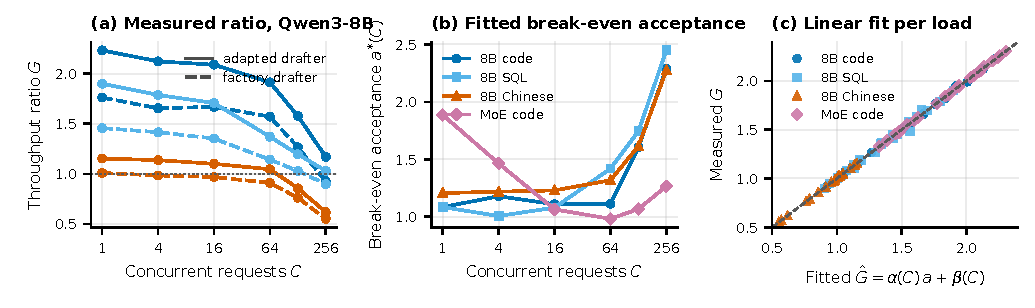
\includegraphics[width=\linewidth]{figures/fig3_frontier.pdf}
\caption{Profitability frontier. (a) Measured speculative over plain throughput for factory (dashed) and adapted (solid) Qwen3-8B drafters; colors as in (b). (b) Fitted break-even acceptance per load. (c) Linear fit versus measurement for all domains and loads.}
\label{fig:frontier}
\end{figure}

\paragraph{Output-length protocol.} Saturated throughput depends on how outputs end (Table~\ref{tab:protocol}). In a batch of 600 requests submitted at once, natural stopping mixes a long drain phase at low concurrency, where speculation is favourable; forcing every output to 256 tokens removes it, and the adapted code drafter then stays below plain decoding. The closed-loop evaluation uses natural stopping, as production traffic does.

\begin{table}[!htbp]
\caption{Code domain, Qwen3-8B: speculative over plain throughput for 600 requests submitted at once, with natural stopping versus outputs forced to 256 tokens.}
\label{tab:protocol}
\centering\small

% Output-length sensitivity across drafter checkpoints
\begingroup
\renewcommand{\arraystretch}{1.22}
\setlength{\tabcolsep}{6pt}

\begin{tabular}{@{}lccc@{}}
\toprule

&
\multicolumn{2}{c}{

  \textbf{Throughput / Plain Decoding}
}
& \\

\cmidrule(lr){2-3}

\textbf{Drafter}
& \textbf{Natural Stop}
& \textbf{Fixed 256 Tokens}
& \textbf{Difference} \\

\midrule

N0
& $0.75\times$
& $0.68\times$
& $-0.06$ \\

N400
& $0.98\times$
& $0.82\times$
& $-0.16$ \\

N800
& $0.88\times$
& $0.83\times$
& $-0.06$ \\

N3200
& \cellcolor{tabGain}
  $\boldsymbol{1.02\times}$
& $0.85\times$
& \cellcolor{tabDrop}
  $\boldsymbol{-0.17}$ \\

\bottomrule
\end{tabular}
\endgroup

\end{table}

\FloatBarrier
\section{Controller Algorithm and Configuration}\label{app:controller}

\paragraph{Prediction model.} The controller predicts from the calibration file alone. With $\Theta_{\mathrm{plain}}(C)$, $T_{\mathrm{base}}(C)$, and $T_{\mathrm{spec}}(C)$ the measured plain throughput and the plain and speculative step times, interpolated in $\log_2 C$ between the calibrated loads, and $g=z\,\Ghat_\ell(a,C)+(1-z)$ the predicted gain of the current speculation state, it predicts the throughput $\Theta(a,z,C,d)=\Theta_{\mathrm{plain}}(C)\,g\,(1-\kappa(C)\,d)$ and the TPOT $\widehat T(a,z,C,d)=T_{\mathrm{base}}(C)/\big(g\,(1-\kappa(C)\,d)\big)$. For a domain without a frontier fit, $\Ghat$ falls back to the proportional form $a\,T_{\mathrm{base}}(C)/T_{\mathrm{spec}}(C)$. The learning curve $a_\ell(N)$ is interpolated in $\log(1+N)$ between the calibrated export points; its inverse gives the requests, and through the domain's mean tokens per request the tokens $n$, that separate $\hat a$ from a target acceptance. In the frozen runs the TPOT entering the rules is this prediction, not a measured latency. Algorithm~\ref{alg:controller} gives one control tick and \cref{tab:constants} the constants.

\begin{algorithm}[!htbp]
\caption{One control tick (every second).}
\label{alg:controller}
\begin{algorithmic}[1]
\STATE Read $C$, the queue, the speculative-decoding counters, and the trainer's state; if more than 20 drafts were made in the last second, $\hat a\leftarrow0.7\,\hat a+0.3\,a_{\mathrm{1s}}$
\IF{the label $\ell$ changed}
\STATE reset the regime clock and $\hat a$, flush the trainer's buffer, restart the export schedule
\ENDIF
\IF{the trainer exported a new drafter}
\STATE hot-swap it; if speculation is off, enable it for 8\,s to measure the new drafter
\ENDIF
\IF{$\ell$ has no learning curve, or $\amax_\ell-\hat a\le0.02$, or the last swap raised $\hat a$ by less than 0.02}
\STATE $d\leftarrow0$
\ELSIF{$\Ghat_\ell(\amax_\ell,C)\le1$}
\STATE $d\leftarrow0$ \COMMENT{structural ceiling}
\ELSIF{predicted TPOT $\le\Tslo$ and the server is not saturated}
\STATE $d\leftarrow$ largest $d\in\mathcal D$ with $T_0/(1-\kappa(C)d)\le0.9\,\Tslo$
\ELSE
\STATE $d\leftarrow\arg\max_{d\in\mathcal D,\,d\le0.5}V(d)$ of \cref{eq:value} if the maximum is positive, else $0$
\ENDIF
\IF{the requests learned in this regime reached the next export point}
\STATE request an export; the next export point doubles the gap (100, 200, 400, \dots)
\ENDIF
\STATE compute $z^{\star}$ by \cref{eq:switch}; switch to $z^{\star}$ if it has differed from $z$ for 3 ticks, the last switch is at least 10\,s old, and no probe is active
\end{algorithmic}
\end{algorithm}

\begin{table}[!htbp]
\caption{Constants of the controller, as fixed in the frozen checkpoint.}
\label{tab:constants}
\centering\small
\begin{tabular}{@{}ll@{}}
\toprule
Constant & Value\\
\midrule
Control period & 1\,s\\
SLO $\Tslo$ & $2\times$ single-request decode time (\nv{slo.m1}\,ms Qwen3-8B, \nv{slo.m2}\,ms MoE)\\
Duty levels $\mathcal D$ & $\{0, 0.1, 0.25, 0.5, 1\}$\\
Slack rule margin & predicted TPOT $\le0.9\,\Tslo$\\
Saturation & queue non-empty, or $C\ge0.95\times256$\\
Duty cap under saturation & 0.5\\
Training target $a^{\dagger}$ & $\hat a+0.8\,(\amax_\ell-\hat a)$\\
Data availability $\rho$ & arrivals plus buffered tokens spread over 10\,s\\
Horizon forecast $\widehat H$ & age of the regime, clipped to $[90,600]$\,s\\
Stop at ceiling & $\amax_\ell-\hat a\le0.02$\\
Stop on convergence & last swap raised $\hat a$ by $<0.02$ (measured $\ge8$\,s after the swap)\\
Speculation switch & 3 agreeing ticks, $\ge10$\,s between switches, 8\,s probe after a swap\\
Export schedule & after 100 requests in the regime, then doubling gaps; $\ge5$\,s between requests\\
Acceptance estimate & moving average with weight 0.3 on the last second (if $>20$ drafts)\\
\bottomrule
\end{tabular}
\end{table}

\FloatBarrier
\section{Baseline Definitions and Fairness}\label{app:policies}

\begin{table}[!htbp]
\caption{The policies of the frozen evaluation. All use the factory drafter at the start of each run.}
\label{tab:policies}
\centering\small
\begin{tabularx}{\linewidth}{@{}l>{\raggedright\arraybackslash}X>{\raggedright\arraybackslash}X>{\raggedright\arraybackslash}X@{}}
\toprule
Policy & Speculation & Training & Information used\\
\midrule
\pol{Production} & always on & none & none (no export, no memory reserve)\\
\pol{Static} & always on & none & none\\
\pol{Plain} & no drafter loaded & none & none\\
\pol{Switch} & \cref{eq:switch} & none & label, frontier\\
\pol{Threshold} & off whenever saturated & duty 0.5 whenever predicted TPOT is within the SLO & load threshold\\
\pol{TIDE} & \cref{eq:switch} & duty 0.5 while collection is on; rounds of 200 requests, keep-if-better, roll back and stop otherwise; re-enabled by acceptance drift & label (frontier only), frontier\\
\pol{Always} & always on & duty 0.5 from the first request; swaps after 100, 200, 400, \dots{} requests & none\\
\pol{Informed} & always on & duty 0.5 from the start of phase B until 800 requests are learned; swaps at 100, 200, 400, 800 & start of phase B; stopping point chosen from the learning curves\\
\pol{Full} & \cref{eq:switch} & \cref{sec:method} & label, frontier, learning curve\\
\bottomrule
\end{tabularx}
\end{table}

\paragraph{Fairness.} All policies except \pol{Production} run the same engine configuration, memory reserve, and export path, serve the same prompt sequence per repetition with the same trainer seed, and start from the factory drafter; they differ only in the information they may use (last column of \cref{tab:policies}) and in what they do with it. \pol{Production} has neither export path nor reserve, so its difference from \pol{Static} is the cost of the infrastructure (\cref{tab:mechanisms}). \pol{Informed} uses information no deployable policy has, the start of phase B and a stopping point read off the learning curves, and is a reference rather than a competitor; \pol{Always} and \pol{Threshold} use less information than \pol{Full}; \pol{Switch} and \pol{TIDE} use the same frontier as \pol{Full} but not the learning curve. The constants of every policy were fixed before the freeze (\cref{sec:limitations}).

\paragraph{The TIDE-style baseline.} \pol{TIDE} reproduces Algorithm~1 of TIDE \citep{park2026tide} in the co-located setting. Its speculation rule is that of \pol{Switch}. Collection is enabled when serving starts. Two moving averages of the measured acceptance length, with weights 0.3 and 0.02 on the newest second and initialised from the first 10 measured seconds, detect a distribution shift when the short one falls more than 0.1 below the long one; a shift re-enables collection. While collection is enabled the trainer runs at duty 0.5, the duty of the other fixed-duty baselines (TIDE itself trains on separate GPUs). After every 200 requests learned the trainer exports a drafter, which is swapped in and measured for 8\,s (with a speculation probe if speculation is off). It is kept if its acceptance is higher than that of the previous drafter just before the swap; otherwise the previous drafter is restored and collection is disabled until the next shift. TIDE leaves the averaging weights, the margin, and the round size unspecified, so these values are ours. TIDE evaluates candidates offline on held-out samples of the round; the frozen trainer has no evaluation path, so we evaluate live, and we declare an evaluation inconclusive, keeping the new drafter, when the traffic label changed within 8\,s before the swap or during the measurement, because the two drafters would then be measured on different traffic. The training rule never uses the label otherwise. \pol{TIDE} was added after the 72-run matrix, on the same frozen checkpoint: its controller and a wrapper that makes the frozen harness start it are new files (\cref{tab:manifest}); no frozen file was changed.

\FloatBarrier
\section{Detailed Serving Results and Decision Ablations}\label{app:extra}

\begin{figure}[!htbp]
\centering
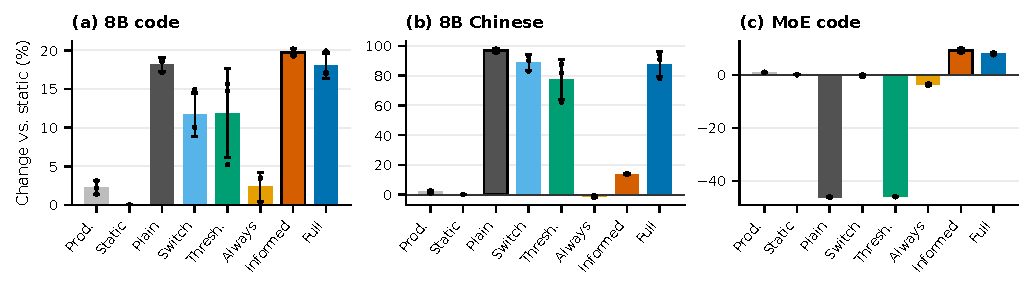
\includegraphics[width=\linewidth]{figures/fig4_policies.pdf}
\caption{Phase-B throughput change relative to \pol{Static} per repetition (dots), with the paired mean and standard deviation (bars). The best policy in each scenario has a black outline. Prod.: \pol{Production}; Thresh.: \pol{Threshold}.}
\label{fig:policies}
\end{figure}

\begin{table}[!htbp]
\caption{Phase-B throughput (tok/s) of every run, the mean, and the coefficient of variation (CV) over the three repetitions.}
\label{tab:runs}
\centering\small

% Per-run throughput results
% Grouped by model architecture and workload
\begingroup
\renewcommand{\arraystretch}{1.15}
\setlength{\tabcolsep}{5pt}

\begin{tabular}{@{}lrrrrr@{}}
\toprule

\textbf{Policy}
& \textbf{Run 1}
& \textbf{Run 2}
& \textbf{Run 3}
& \textbf{Mean}
& \textbf{CV} \\

\midrule

% ===== Qwen3-8B: Code =====
\rowcolor{tabGroup}
\multicolumn{6}{@{}l@{}}{%
  \textbf{Qwen3-8B (Dense) -- Code}
} \\

Production speculation
& 14{,}590 & 14{,}672 & 14{,}541
& 14{,}601 & 0.5\% \\

Static speculation
& 14{,}392 & 14{,}229 & 14{,}224
& 14{,}282 & 0.7\% \\

Plain decoding
& 16{,}851 & 16{,}861 & 16{,}896
& 16{,}869 & 0.1\% \\

Switch only
& 16{,}537 & 15{,}660 & 16{,}162$^\dagger$
& 16{,}120 & 2.7\% \\

Threshold rule
& 16{,}419$^\dagger$ & 16{,}330 & 16{,}450
& 16{,}400 & 0.4\% \\

TIDE-style triggers
& 16{,}246 & 15{,}780 & 16{,}733
& 16{,}253 & 2.9\% \\

Always train
& 14{,}417 & 14{,}724 & 14{,}709
& 14{,}617 & 1.2\% \\

Informed schedule
& 17{,}247 & 17{,}096 & 16{,}963
& \cellcolor{tabBest}\textbf{17{,}102}
& 0.8\% \\

\rowcolor{tabFull}
\textbf{Full controller}
& 16{,}831 & 16{,}674 & 17{,}054
& \textbf{16{,}853} & 1.1\% \\

\addlinespace[4pt]

% ===== Qwen3-8B: Chinese =====
\rowcolor{tabGroup}
\multicolumn{6}{@{}l@{}}{%
  \textbf{Qwen3-8B (Dense) -- Chinese}
} \\

Production speculation
& 8{,}675 & 8{,}677 & 8{,}694
& 8{,}682 & 0.1\% \\

Static speculation
& 8{,}494 & 8{,}594 & 8{,}491
& 8{,}526 & 0.7\% \\

Plain decoding
& 16{,}795 & 16{,}793 & 16{,}793
& \cellcolor{tabBest}\textbf{16{,}794}
& 0.0\% \\

Switch only
& 16{,}149 & 16{,}256$^\dagger$ & 16{,}414
& 16{,}273 & 0.8\% \\

Threshold rule
& 15{,}928 & 15{,}639 & 16{,}242$^\dagger$
& 15{,}936 & 1.9\% \\

TIDE-style triggers
& 13{,}140 & 13{,}572 & 12{,}797
& 13{,}170 & 2.9\% \\

Always train
& 8{,}406 & 8{,}432 & 8{,}442
& 8{,}427 & 0.2\% \\

Informed schedule
& 9{,}691 & 9{,}781 & 9{,}624
& 9{,}699 & 0.8\% \\

\rowcolor{tabFull}
\textbf{Full controller}
& 16{,}214 & 15{,}301 & 16{,}475
& \textbf{15{,}997} & 3.9\% \\

\addlinespace[4pt]

% ===== Qwen3-30B-A3B: MoE Code =====
\rowcolor{tabGroup}
\multicolumn{6}{@{}l@{}}{%
  \textbf{Qwen3-30B-A3B (MoE) -- Code}
} \\

Production speculation
& 13{,}990 & 13{,}986 & 14{,}000
& 13{,}992 & 0.0\% \\

Static speculation
& 13{,}847 & 13{,}861 & 13{,}870
& 13{,}859 & 0.1\% \\

Plain decoding
& 7{,}472 & 7{,}466 & 7{,}458
& 7{,}465 & 0.1\% \\

Switch only
& 13{,}839 & 13{,}770 & 13{,}841
& 13{,}816 & 0.3\% \\

Threshold rule
& 7{,}486 & 7{,}485 & 7{,}496
& 7{,}489 & 0.1\% \\

TIDE-style triggers
& 14{,}803 & 15{,}174$^\dagger$ & 14{,}101
& 14{,}692 & 3.7\% \\

Always train
& 13{,}372 & 13{,}324 & 13{,}396
& 13{,}364 & 0.3\% \\

Informed schedule
& 15{,}217 & 15{,}183 & 15{,}054
& \cellcolor{tabBest}\textbf{15{,}151}
& 0.6\% \\

\rowcolor{tabFull}
\textbf{Full controller}
& 14{,}965 & 15{,}018 & 14{,}920
& \textbf{14{,}967} & 0.3\% \\

\bottomrule
\end{tabular}
\endgroup

\end{table}

\begin{table}[!htbp]
\caption{Per-run behaviour of \pol{Full} during phase B, and the node each run used.}
\label{tab:fullruns}
\centering\small

% Per-run controller behavior
% Grouped by model architecture and workload
\begingroup
\renewcommand{\arraystretch}{1.18}
\setlength{\tabcolsep}{4pt}

\begin{tabular}{@{}
    c
    r
    >{\columncolor{tabLoad}}r
    c
    c
    c
    r
    l@{}}
\toprule

\textbf{Run}
& \textbf{B tok/s}
& \textbf{Spec.\ on}
& \textbf{Duty}
& \textbf{Swaps}
& \textbf{Final acc.}
& \shortstack{\textbf{Train tok.}\\\textbf{(M)}}
& \textbf{Node} \\

\midrule

% ===== Qwen3-8B: Code =====
\rowcolor{tabGroup}
\multicolumn{8}{@{}l@{}}{%
  \textbf{Qwen3-8B (Dense) -- Code}
} \\

1 & 16{,}831 & 100\%
  & 0.079 & 3 & 2.65 & 0.74 & c0803 \\

2 & 16{,}674 & 100\%
  & 0.074 & 3 & 2.67 & 0.67 & c0806 \\

3 & 17{,}054 & 100\%
  & 0.050 & 3 & 2.67 & 0.50 & c0806 \\

\addlinespace[3pt]

% ===== Qwen3-8B: Chinese =====
\rowcolor{tabGroup}
\multicolumn{8}{@{}l@{}}{%
  \textbf{Qwen3-8B (Dense) -- Chinese}
} \\

1 & 16{,}214
  & \cellcolor{tabHighlight}\textbf{2\%}
  & 0.018 & 1 & 1.20 & 0.39 & c0803 \\

2 & 15{,}301
  & \cellcolor{tabHighlight}\textbf{2\%}
  & 0.013 & 1 & 1.18 & 0.36 & c0803 \\

3 & 16{,}475
  & \cellcolor{tabHighlight}\textbf{1\%}
  & 0.017 & 1 & 1.17 & 0.39 & c0812 \\

\addlinespace[3pt]

% ===== Qwen3-30B-A3B: MoE Code =====
\rowcolor{tabGroup}
\multicolumn{8}{@{}l@{}}{%
  \textbf{Qwen3-30B-A3B (MoE) -- Code}
} \\

1 & 14{,}965 & 100\%
  & 0.075 & 4 & 2.97 & 0.71 & c0813 \\

2 & 15{,}018 & 100\%
  & 0.079 & 4 & 2.99 & 0.72 & c0812 \\

3 & 14{,}920 & 100\%
  & 0.098 & 4 & 2.97 & 0.99 & c0803 \\

\bottomrule
\end{tabular}
\endgroup

\end{table}

\paragraph{Latency.}\label{app:latency} Table~\ref{tab:latency} gives TPOT per phase. In phase A2, \pol{Full} stays close to \pol{Static} on Qwen3-8B (\nv{code.full.a2}\%, \nv{zh.full.a2}\%) because it keeps training in the slack, whereas \pol{Informed}, which has stopped training and kept its adapted drafter, changes A2 TPOT by \nv{code.informed.a2}\% and \nv{zh.informed.a2}\%. On the MoE target the calibration contains no chat learning curve, so \pol{Full} never trains in the chat phases, and its code-adapted drafter changes A2 TPOT by \nv{moe.full.a2}\% (\pol{Informed}: \nv{moe.informed.a2}\%). A latency-oriented deployment would cap the duty of the slack rule.

\begin{table}[!htbp]
\caption{TPOT in milliseconds (means over three runs): median in the light chat phases A1 and A2, and 99th percentile in the saturated phase B.}
\label{tab:latency}
\centering\small

% Latency comparison -- grouped by model architecture
\begingroup
\renewcommand{\arraystretch}{1.20}
\setlength{\tabcolsep}{3pt}

\begin{tabular}{@{}l*{9}{r}@{}}
\toprule

% ===== Model architecture groups =====
&
\multicolumn{6}{c}{
  \textbf{Qwen3-8B (Dense)}
}
&
\multicolumn{3}{c}{
  \textbf{30B-A3B (MoE)}
} \\

\cmidrule(lr){2-7}
\cmidrule(l){8-10}

% ===== Workload groups =====
&
\multicolumn{3}{c}{\textbf{Code}}
&
\multicolumn{3}{c}{\textbf{Chinese}}
&
\multicolumn{3}{c}{\textbf{Code}} \\

\cmidrule(lr){2-4}
\cmidrule(lr){5-7}
\cmidrule(l){8-10}

% ===== Latency metrics =====
\textbf{Policy}
& \textbf{A1 p50}
& \textbf{B p99}
& \textbf{A2 p50}
& \textbf{A1 p50}
& \textbf{B p99}
& \textbf{A2 p50}
& \textbf{A1 p50}
& \textbf{B p99}
& \textbf{A2 p50} \\

\midrule

Static speculation
& 5.77 & 22.01 & 5.66
& 5.70 & 36.54 & 5.69
& 11.17 & 23.42 & 11.09 \\

Plain decoding
& 8.92
& \cellcolor{tabBest}\textbf{15.08}
& 8.92
& 8.92
& \cellcolor{tabBest}\textbf{15.35}
& 8.86
& 16.61 & 33.83 & 16.53 \\

Switch only
& 5.69 & 17.27 & 5.65
& 5.70 & 18.84 & 5.73
& 11.13 & 23.52 & 11.11 \\

Informed schedule
& 5.77 & 22.88 & 4.74
& 5.77 & 37.41 & 5.06
& 11.28 & 22.69 & 10.19 \\

\addlinespace[3pt]

% ===== Proposed controller =====
\rowcolor{tabFull}
\textbf{Full controller}
& 6.35 & 20.88 & 5.56
& 6.36 & 18.44 & 5.85
& 11.07
& \cellcolor{tabBest}\textbf{22.58}
& 10.04 \\

\bottomrule
\end{tabular}
\endgroup

\end{table}

\IfFileExists{tables/tab_tide.tex}{\begin{table}[!htbp]
\caption{What \pol{TIDE} did (means over three runs): speculation-on and training shares of phase B, mean duty cycle in B, evaluated rounds (kept, inconclusive, rejected), drift triggers, and tokens trained over the whole run.}
\label{tab:tide}
\centering\small\setlength{\tabcolsep}{4pt}

% TIDE-style controller behavior
% Grouped by model architecture
\begingroup
\renewcommand{\arraystretch}{1.20}
\setlength{\tabcolsep}{3pt}

\begin{tabular}{@{}lccccccc@{}}
\toprule

\textbf{Scenario}
& \shortstack{\textbf{Spec.}\\\textbf{on}}
& \textbf{Training}
& \textbf{Duty}
& \textbf{Rounds}
& \shortstack{\textbf{Kept / Inconcl.}\\\textbf{/ Rejected}}
& \textbf{Drifts}
& \shortstack{\textbf{Tokens}\\\textbf{(M)}} \\

\midrule

% ===== Qwen3-8B (Dense) =====
\rowcolor{tabGroup}
\multicolumn{8}{@{}l@{}}{%
  \textbf{Qwen3-8B (Dense)}
} \\

Code
& 100\%
& 38\%
& 0.106
& 8.0
& 4.7 / 1.7 / 1.7
& 1.7
& 1.25 \\

Chinese
& \cellcolor{tabHighlight}\textbf{16\%}
& \cellcolor{tabHighlight}\textbf{70\%}
& \cellcolor{tabHighlight}\textbf{0.299}
& 8.3
& 4.3 / 1.0 / 3.0
& 2.3
& 0.53 \\

\addlinespace[3pt]

% ===== Qwen3-30B-A3B (MoE) =====
\rowcolor{tabGroup}
\multicolumn{8}{@{}l@{}}{%
  \textbf{Qwen3-30B-A3B (MoE)}
} \\

Code
& 100\%
& 26\%
& 0.038
& 4.3
& 1.0 / 1.3 / 2.0
& 2.0
& 0.72 \\

\bottomrule
\end{tabular}
\endgroup

\end{table}}{}

\IfFileExists{tables/app_tidevar.tex}{\paragraph{Sensitivity of \pol{TIDE}.}\label{app:tidevar} TIDE leaves its round size and drift margin open (\cref{app:policies}). We reran \pol{TIDE} with rounds of \nv{tv.round} requests, four times larger, and a drift margin of \nv{tv.eps}, three times larger, everything else unchanged, on the same checkpoint, prompts, and seeds; the interference scan of \cref{app:rerun} flags \nv{tv.scan.flagged} of these nine runs. On Chinese the larger margin removes the drift triggers (\nv{zh.tv.drift} per run instead of \nv{zh.tide.drift}), but each larger round still raises acceptance a little, so the keep-if-better test keeps training going for \nv{zh.tv.trainB}\% of phase B, and \pol{Full} stays ahead in every repetition (\nv{zh.full_vs_tv.min} to \nv{zh.full_vs_tv.max}\%). On the code scenarios the larger rounds bring \pol{TIDE} to within \nv{code.full_vs_tv}\% (Qwen3-8B) and \nv{moe.full_vs_tv}\% (MoE) of \pol{Full}. Its worst case over the three scenarios becomes \nv{tv.worst} of the best policy, against \nv{full.worst} for \pol{Full} and \nv{switch.worst} for \pol{Switch} (\cref{tab:tidevar}).

\begin{table}[!htbp]
\caption{\pol{TIDE} with its default setting (rounds of 200 requests, drift margin 0.1) and with rounds of \nv{tv.round} requests and margin \nv{tv.eps} (means over three runs): phase-B throughput, paired difference of \pol{Full} against it, share of phase B spent training, evaluated rounds (kept, inconclusive, rejected), and drift triggers.}
\label{tab:tidevar}
\centering\small\setlength{\tabcolsep}{4pt}

% TIDE-style baseline -- parameter sensitivity
% Grouped by model architecture
\begingroup
\renewcommand{\arraystretch}{1.20}
\setlength{\tabcolsep}{3.5pt}

\begin{tabular}{@{}llrrrrcr@{}}
\toprule

\textbf{Scenario}
& \shortstack{\textbf{Round /}\\\textbf{Margin}}
& \shortstack{\textbf{B}\\\textbf{tok/s}}
& \shortstack{\textbf{\pol{Full}}\\\textbf{vs.\ TIDE}}
& \shortstack{\textbf{Training}\\\textbf{(B)}}
& \textbf{Rounds}
& \shortstack{\textbf{Kept / Inconcl.}\\\textbf{/ Rejected}}
& \textbf{Drifts} \\

\midrule

% ===== Qwen3-8B (Dense) =====
\rowcolor{tabGroup}
\multicolumn{8}{@{}l@{}}{%
  \textbf{Qwen3-8B (Dense)}
} \\

Code
& 200 / 0.1
& 16{,}253
& $+3.7\%$
& 38\%
& 8.0
& 4.7 / 1.7 / 1.7
& 1.7 \\

\rowcolor{tabLoad}
&
  800 / 0.3
& 16{,}514
& $+2.1\%$
& 47\%
& 3.0
& 2.0 / 0.0 / 1.0
& 1.0 \\

\addlinespace[3pt]

Chinese
& 200 / 0.1
& 13{,}170
& \cellcolor{tabHighlight}
  $\boldsymbol{+21.6\%}$
& 70\%
& 8.3
& 4.3 / 1.0 / 3.0
& 2.3 \\

\rowcolor{tabLoad}
&
  800 / 0.3
& 14{,}484
& \cellcolor{tabHighlight}
  $\boldsymbol{+10.7\%}$
& 51\%
& 3.3
& 2.3 / 0.0 / 1.0
& 0.0 \\

\addlinespace[3pt]

% ===== Qwen3-30B-A3B (MoE) =====
\rowcolor{tabGroup}
\multicolumn{8}{@{}l@{}}{%
  \textbf{Qwen3-30B-A3B (MoE)}
} \\

Code
& 200 / 0.1
& 14{,}692
& $+2.0\%$
& 26\%
& 4.3
& 1.0 / 1.3 / 2.0
& 2.0 \\

\rowcolor{tabLoad}
&
  800 / 0.3
& 14{,}887
& $+0.5\%$
& 36\%
& 3.3
& 2.3 / 0.0 / 1.0
& 1.0 \\

\bottomrule
\end{tabular}
\endgroup

\end{table}}{}

\begin{table}[!htbp]
\caption{Costs of the mechanisms, measured inside the frozen runs.}
\label{tab:mechanisms}
\centering\small

% Runtime overheads -- grouped by mechanism
\begingroup
\renewcommand{\arraystretch}{1.20}
\setlength{\tabcolsep}{4pt}

\begin{tabularx}{\linewidth}{@{}
    >{\raggedright\arraybackslash}p{0.27\linewidth}
    >{\raggedright\arraybackslash}p{0.33\linewidth}
    >{\raggedright\arraybackslash}X
    @{}}
\toprule

\textbf{Mechanism}
& \textbf{Measurement}
& \textbf{Result} \\

\midrule

% ===== Serving overheads =====
\rowcolor{tabGroup}
\multicolumn{3}{@{}l@{}}{%
  \textbf{\footnotesize Serving Overheads}
} \\

Feature export + trainer memory reserve
& Production vs.\ static speculation,
  saturated throughput
& 8B code 2.2\%,
  8B Chinese 1.8\%,
  MoE code 1.0\% \\

Runtime-off state vs.\ no drafter
& Switch only vs.\ plain decoding,
  saturated throughput
& \cellcolor{tabHighlight}
  \textbf{8B code $-4.4$\%,
  8B Chinese $-3.1$\%} \\

\addlinespace[3pt]

% ===== Runtime operations =====
\rowcolor{tabGroup}
\multicolumn{3}{@{}l@{}}{%
  \textbf{\footnotesize Runtime Operations}
} \\

Drafter hot swap (8B)
& 181 swaps in the frozen runs
& Median 0.71\,s,
  range 0.33--1.58\,s \\

Drafter hot swap (MoE)
& 70 swaps in the frozen runs
& Median 0.31\,s,
  range 0.21--0.76\,s \\

Speculation switch
& 74 switches, RPC round trip
& Median 22\,ms,
  max.\ 66\,ms \\

\addlinespace[3pt]

% ===== Training data usage =====
\rowcolor{tabGroup}
\multicolumn{3}{@{}l@{}}{%
  \textbf{\footnotesize Training Data Usage}
} \\

\rowcolor{tabFull}
\textbf{Training data used (full controller)}
& Requests consumed by the trainer,
  of 16{,}400 served per run
& 8B code 1{,}746 (11\%),
  8B Chinese 849 (5\%),
  MoE code 2{,}648 (16\%) \\

\bottomrule
\end{tabularx}
\endgroup

\end{table}

\FloatBarrier
\subsection{Decision ablations: which test the gain comes from}\label{app:ablation}

The policies of \cref{tab:main} are partial ablations, but none isolates the payback rule, and \pol{Switch} removes training altogether. We therefore reran \pol{Full} with one of its tests removed, on the frozen checkpoint, prompts, and seeds (\nv{abl.n.runs} runs; \cref{tab:ablate} in \cref{sec:levers}): \emph{without the payback rule}, the trainer runs at duty 0.5 whenever the stop tests allow it under saturation; \emph{without the stop tests}, the structural-ceiling, at-ceiling, and convergence tests are skipped; \emph{without the switch}, speculation stays on and training is valued with speculation stuck on (\cref{app:controller}); \emph{without per-domain knowledge}, the controller ignores the traffic label and the learning curves: it predicts throughput with the per-target proportional frontier $\Ghat(a,C)=a\,T_{\mathrm{base}}(C)/T_{\mathrm{spec}}(C)$, assumes that the next round raises acceptance by 0.3, replaces that prior with the gain measured after every swap, and, after a round that did not pay, waits 120\,s before trying one more.

The gain comes from a different test in each scenario. On Chinese it comes entirely from the switch (\nv{abl.noswitch.zh.vsv6}\% without it, \nv{abl.noswitch.zh.min} to \nv{abl.noswitch.zh.max}\% per repetition), while the other three variants stay within noise of \pol{Full}. On Qwen3-8B code it comes from training, and the payback rule is worth \nv{abl.novalue.code.vsv6.abs}\% there: at a fixed duty the trainer runs until the ceiling test stops it (mean duty \nv{abl.novalue.code.duty} against \nv{code.full.duty}), and the interference costs more than the last drafters gain. On the MoE target every variant trains and stops at the ceiling, and no single test is decisive. The stop tests change nothing under saturation (\nv{abl.nostop.code.vsv6}\%, \nv{abl.nostop.zh.vsv6}\%, \nv{abl.nostop.moe.vsv6}\%): near the ceiling the payback rule already finds no value, and on Chinese it finds none even without the structural-ceiling test, so the three tests are shortcuts that matter only for the SLO-slack rule in the light phases. The variant without per-domain knowledge stays within noise of \pol{Full} in all three scenarios (\nv{abl.nocurve.code.vsv6}\%, \nv{abl.nocurve.zh.vsv6}\%, \nv{abl.nocurve.moe.vsv6}\%): the switch needs only the measured acceptance and the per-target step times, and the measured swap gains replace the learning curve. Its one cost is timing: in one Chinese repetition (\nv{abl.nocurve.zh.min}\%) a drafter trained in the slack reached its export point late in phase B, and the speculation probe after the swap ran at saturation on Chinese. Where the curves matter is traffic that a label does not describe, which \cref{app:mix} examines.


\FloatBarrier
\section{Mixed-Traffic and Calibration Robustness}\label{app:mix}

\begin{table}[t]
\caption{Mixed traffic on the frozen Qwen3-8B checkpoint: phase B serves a request-level 50/50 mixture of two domains. Phase-B throughput relative to \pol{Static} (paired mean $\pm$ standard deviation over three repetitions) and, in parentheses, the ratio to the best policy of the column.}
\label{tab:mix}
\centering\small
\IfFileExists{tables/app_mix.tex}{
% Mixed-traffic results -- grouped by model and policy type
\begingroup
\renewcommand{\arraystretch}{1.20}
\setlength{\tabcolsep}{5pt}

\begin{tabular}{@{}lcc@{}}
\toprule

% ===== Model group =====
&
\multicolumn{2}{c}{
  \textbf{Qwen3-8B (Dense)}
} \\
\cmidrule(l){2-3}

\textbf{Policy}
& \textbf{Code + Chat}
& \textbf{Chinese + Chat} \\
\midrule

% ===== Baseline policies =====
\rowcolor{tabGroup}
\multicolumn{3}{@{}l}{
  \textbf{\footnotesize Baseline Policies}
} \\

Static
& 12{,}748 tok/s\,{\scriptsize(0.822)}
& 10{,}138 tok/s\,{\scriptsize(0.650)} \\

Plain
& \cellcolor{tabBest}
  $\boldsymbol{+21.7\pm0.6}$\,
  {\scriptsize\bfseries(1.000)}
& \cellcolor{tabBest}
  $\boldsymbol{+53.7\pm0.4}$\,
  {\scriptsize\bfseries(1.000)} \\

Switch
& $+19.3\pm0.4$\,{\scriptsize(0.980)}
& $+50.0\pm0.7$\,{\scriptsize(0.976)} \\

TIDE
& $+16.9\pm0.5$\,{\scriptsize(0.961)}
& $+44.8\pm2.9$\,{\scriptsize(0.942)} \\

\addlinespace[3pt]

% ===== Proposed controller and variants =====
\rowcolor{tabGroup}
\multicolumn{3}{@{}l}{
  \textbf{\footnotesize Proposed Controller and Variants}
} \\

\rowcolor{tabFull}
\textbf{Full}
& $+16.0\pm2.1$\,{\scriptsize(0.953)}
& $+50.4\pm0.3$\,{\scriptsize(0.978)} \\

Full, stale label
& $+14.7\pm0.5$\,{\scriptsize(0.942)}
& $+48.3\pm0.4$\,{\scriptsize(0.965)} \\

Full, label-free
& $+13.0\pm3.6$\,{\scriptsize(0.928)}
& $+50.0\pm1.0$\,{\scriptsize(0.976)} \\

\bottomrule
\end{tabular}
\endgroup
}{}
\end{table}

The live workloads of \cref{tab:main} switch between single domains, and the controller is told which one it serves. Production traffic is often a mixture without a clean switch point, and the label can be stale. We therefore built two mixtures by interleaving, request by request, equal numbers of prompts from two pools, code with chat and Chinese with chat, and ran the policies of \cref{tab:main} on them with the same phases, seeds, and harness (\nv{mix.n.runs} runs). Each mixture was calibrated as a domain of its own by the profiling runs of \cref{app:calibration}: the code--chat drafter learns from an acceptance of \nv{mix.cc.acc0} to a ceiling of \nv{mix.cc.ceiling}, which at $C{=}256$ moves it from \nv{mix.cc.gain.n0.c256}$\times$ to \nv{mix.cc.gain.n3200.c256}$\times$ plain decoding on the calibrated frontier (break-even at \nv{mix.cc.breakeven.c256}); the Chinese--chat drafter learns from \nv{mix.zc.acc0} to \nv{mix.zc.ceiling} and stays below plain decoding (\nv{mix.zc.gain.n0.c256}$\times$ to \nv{mix.zc.gain.n3200.c256}$\times$). Two further variants of \pol{Full} test the label: with a \emph{stale label} the controller is told that phase B is still chat, so it uses chat's curve and frontier on the mixture's prompts; the \emph{label-free} variant of \cref{app:ablation} has neither label nor curve.

Neither mixture pays for speculation at saturation, so \cref{tab:mix} ranks the policies by how much each loses on the way to that conclusion, and plain decoding is the best policy on both. On Chinese--chat the structural-ceiling test fires on the first tick of phase B: \pol{Full} turns speculation off (on for \nv{mix.zc.v6.spec}\% of the phase), does not train on the mixture (mean duty \nv{mix.zc.v6.duty}), and ends \nv{mix.zc.v6.vsnospec}\% from \pol{Plain}, the cost of the speculation-off state (\cref{tab:mechanisms}), and within noise of \pol{Switch} (\nv{mix.zc.v6.vsswitch}\%). The label-free variant reaches the same decision from the measured acceptance (\nv{mix.zc.v6_nocurve.vsv6}\% from \pol{Full}). With the stale label the controller believes it serves chat, trains one round, swaps the drafter in, finds no gain, and stops; the wasted round costs \nv{mix.zc.v6_stale.vsv6.abs}\% in every repetition. \pol{TIDE} re-enables training on every drift it measures, swaps \nv{mix.zc.tide.swaps} drafters, and ends \nv{mix.zc.tide.vsv6}\% from \pol{Full}. Code--chat is a break-even mixture: the adapted drafter's ceiling is just above the break-even acceptance, so what it can return is within the error of the calibration, and every policy except \pol{Static} lands within \nv{mix.cc.band}\% of \pol{Plain}. \pol{Full} trains \nv{mix.cc.v6.swaps} rounds on average, stops when a swap no longer raises acceptance or the payback rule finds nothing left to earn, and keeps speculation on (\nv{mix.cc.v6.spec}\% of the phase) because the calibrated frontier predicts a small gain at the acceptance it reaches; the rounds that get it there and the part of the phase served by the factory drafter cost more than the adapted drafter returns, and it ends \nv{mix.cc.v6.vsswitch}\% behind \pol{Switch}, which turns speculation off at the factory drafter's acceptance, and \nv{mix.cc.v6.vsnospec}\% behind \pol{Plain}. Here the curve is worth something: the label-free variant expects every round to raise acceptance by its prior and trains for longer (mean duty \nv{mix.cc.v6_nocurve.duty} against \nv{mix.cc.v6.duty}, \nv{mix.cc.v6_nocurve.swaps} swaps) before the measured swap gains stop it, and pays \nv{mix.cc.v6_nocurve.vsv6.abs}\% more than \pol{Full}; the stale label costs \nv{mix.cc.v6_stale.vsv6.abs}\%, within noise.

Two caveats. The proportion of each mixture is fixed throughout phase B, because the benchmark client shuffles each prompt pool; a mixture whose proportion drifts within a regime is not covered. And on a break-even mixture the right decision is within the calibration error, so no policy that speculates can be expected to beat plain decoding there; what the controller contributes is to lose little (\nv{mix.cc.v6.r} of the best policy) rather than to win.


\FloatBarrier
\section{Cross-Engine Implementation and Results: SGLang}\label{app:sglang}

\paragraph{Port.} We reimplemented the three engine extensions of \cref{sec:system} on SGLang 0.5.10 \citep{zheng2024sglang}, as a runtime patch of its default EAGLE-3 path, which runs without SGLang's overlap scheduler. The live tap writes the records of \cref{sec:system} to the same ring buffer, so the trainer is unchanged; its rows are the prefill chunks, the accepted prefix of every verification, and the input token of every step with speculation off. A drafter swap copies the exported weights in place, skipping the embedding that the drafter shares with the target. With speculation off, a decode step runs the target on a second set of CUDA graphs, captured at start-up for plain decoding, with the bookkeeping of a verification that accepted no draft. As in vLLM, the drafter does not run while speculation is off; the first speculative step afterwards refreshes the drafter's inputs with one pass over every request's last committed position. A metrics endpoint with vLLM's names and an RPC endpoint let the harness, benchmark client, controller, trainer, prompt files, and seeds of the vLLM checkpoint run unchanged, with identical hashes.

\paragraph{Checks.} Before calibrating we checked the port on both targets. Greedy outputs with speculation on and off agreed on \nv{sgl.8b.greedy} prompts for Qwen3-8B and \nv{sgl.moe.greedy} for the MoE target. Toggling speculation every 0.5\,s under load (\nv{sgl.8b.flips} and \nv{sgl.moe.flips} toggles) completed every request with exact token counts. Swapping drafters moved Qwen3-8B's acceptance on code from \nv{sgl.8b.acc.factory} (factory) to \nv{sgl.8b.acc.trained} (a code drafter from the vLLM runs) and \nv{sgl.8b.acc.zero} (its input layer zeroed), and back to \nv{sgl.8b.acc.back}, without changing the target's output. The exported hidden states match those of Hugging Face Transformers row by row, with cosine similarity at least \nv{sgl.8b.cosmin} for Qwen3-8B and \nv{sgl.moe.cosmin} for the MoE target.

\begin{table}[t]
\caption{SGLang output throughput (tokens/s) on code prompts: one speculative server with speculation on (acceptance in parentheses) and switched off, and a server without a drafter with and without SGLang's overlap scheduler. --: not measured.}
\label{tab:sgl_speed}
\centering\small
\IfFileExists{tables/app_sgl_speed.tex}{
% SGLang execution-mode throughput comparison
% Grouped by model architecture and execution mode
\begingroup
\renewcommand{\arraystretch}{1.20}
\setlength{\tabcolsep}{5pt}

\begin{tabular}{@{}crrrr@{}}
\toprule

% ===== Execution-mode groups =====
&
\multicolumn{2}{c}{
  \textbf{Drafter Loaded}
}
&
\multicolumn{2}{c}{
  \textbf{Plain Decoding}
} \\

\cmidrule(lr){2-3}
\cmidrule(l){4-5}

\textbf{$C$}
& \shortstack{\textbf{Spec. On}\\\textbf{(Acc.)}}
& \shortstack{\textbf{Spec. Off}}
& \shortstack{\textbf{Plain}\\\textbf{Server}}
& \shortstack{\textbf{Plain,}\\\textbf{No Overlap}} \\

\midrule

% ===== Qwen3-8B (Dense) =====
\rowcolor{tabGroup}
\multicolumn{5}{@{}l@{}}{%
  \textbf{Qwen3-8B (Dense)}
} \\

1
& 188 (2.14)
& 111
& 117
& 115 \\

16
& 1{,}874 (2.11)
& 1{,}254
& 1{,}341
& 1{,}360 \\

64
& 5{,}503 (2.14)
& 3{,}941
& 4{,}314
& 4{,}093 \\

\rowcolor{tabLoad}
\textbf{256}
& 10{,}538 (2.13)
& \cellcolor{tabHighlight}\textbf{9{,}430}
& \textbf{11{,}152}
& 10{,}000 \\

\addlinespace[4pt]

% ===== Qwen3-30B-A3B (MoE) =====
\rowcolor{tabGroup}
\multicolumn{5}{@{}l@{}}{%
  \textbf{Qwen3-30B-A3B (MoE)}
} \\

1
& 259 (2.64)
& 171
& 185
& 175 \\

16
& 1{,}181 (2.60)
& 736
& 766
& 731 \\

64
& 2{,}556 (2.63)
& 1{,}705
& 1{,}833
& 1{,}716 \\

\rowcolor{tabLoad}
\textbf{256}
& 6{,}729 (2.64)
& \cellcolor{tabHighlight}\textbf{3{,}803}
& \textbf{4{,}274}
& -- \\

\bottomrule
\end{tabular}
\endgroup
}{}
\end{table}

\paragraph{A step without speculation costs more than in vLLM.} In vLLM, switching speculation off on Qwen3-8B code at concurrency 256 raised throughput by \nv{vllm.off_vs_on.c256}\% over speculating, and in the frozen matrix its speculation-off state was \nv{zh.switch_vs_plain.abs}--\nv{code.switch_vs_plain.abs}\% slower than plain decoding (\cref{tab:mechanisms}). In SGLang, a step with speculation switched off is \nv{sgl.off_vs_plain.c256}\% slower than a server without a drafter (Table~\ref{tab:sgl_speed}). About \nv{sgl.nooverlap.c256} points come from the overlap scheduler, which SGLang's speculative path does not use (a plain server without it is that much slower), and \nv{sgl.port.c256} points from the bookkeeping of the speculative path. Switching off therefore loses \nv{sgl.on_vs_off.c256}\% against speculating on Qwen3-8B code, while a plain server would gain \nv{sgl.plain_vs_on.c256}\%. A first version that kept the drafter current at every step with speculation off was \nv{sgl.v1off_vs_plain.c256}\% slower than a plain server; we replaced it before calibrating.

\paragraph{Calibration and checkpoint.} SGLang was calibrated with the same scripts and prompts (load sweep, interference at duty 0.1 to 1, frontier with the same drafter checkpoints). Plain decoding in the calibration is the speculative server with speculation switched off, since that is what the controller obtains by setting $z{=}0$; the plain server is the \pol{Plain} baseline. The learning curves are those of \cref{sec:measure}, since drafters and prompts are the same. vLLM's memory utilisation $u$, which caps the whole server, maps to SGLang's static fraction $u$ minus the server's measured non-static memory, so the server's peak footprint and the trainer's reserve are those of the vLLM runs. The SGLang runs use their own checkpoint, frozen after calibration and before the first run (Table~\ref{tab:sgl_manifest}).

\begin{table}[t]
\caption{SGLang: phase-B throughput change relative to \pol{Static} (paired mean $\pm$ standard deviation over three repetitions; ratio to the best policy of the scenario in parentheses; best policy in bold). Last column: the worst ratio across scenarios.}
\label{tab:sgl_main}
\centering\small
\IfFileExists{tables/app_sgl_main.tex}{
% SGLang performance -- grouped by model architecture
\begingroup
\renewcommand{\arraystretch}{1.18}
\setlength{\tabcolsep}{3pt}

\begin{tabular}{@{}lcccc@{}}
\toprule

% ===== Model architecture groups =====
&
\multicolumn{2}{c}{
  \textbf{Qwen3-8B (Dense)}
}
&
\multicolumn{1}{c}{
  \shortstack{
    \textbf{30B-A3B}
    \textbf{(MoE)}
  }
}
& \\

\cmidrule(lr){2-3}
\cmidrule(lr){4-4}

\textbf{Policy}
& \textbf{Code}
& \textbf{Chinese}
& \textbf{Code}
& \textbf{Worst case} \\

\midrule

% ===== Serving baselines =====
Static speculation
& 10{,}402 tok/s\,{\scriptsize(0.862)}
& 6{,}422 tok/s\,{\scriptsize(0.523)}
& 6{,}800 tok/s\,{\scriptsize(0.923)}
& 0.523 \\

Plain decoding
& \cellcolor{tabBest}
  $\boldsymbol{+16.0\pm0.6}$\,
  {\scriptsize\bfseries(1.000)}
& \cellcolor{tabBest}
  $\boldsymbol{+91.4\pm0.9}$\,
  {\scriptsize\bfseries(1.000)}
& $-31.9\pm0.5$\,{\scriptsize(0.628)}
& 0.628 \\

\addlinespace[2pt]

% ===== Adaptive policies =====
Switch only
& $-0.5\pm0.2$\,{\scriptsize(0.858)}
& $+37.9\pm3.9$\,{\scriptsize(0.721)}
& $-0.7\pm0.9$\,{\scriptsize(0.917)}
& \cellcolor{tabBest}\textbf{0.721} \\

TIDE-style triggers
& $+15.8\pm1.0$\,{\scriptsize(0.999)}
& $+35.8\pm1.6$\,{\scriptsize(0.710)}
& \cellcolor{tabBest}
  $\boldsymbol{+8.4\pm1.0}$\,
  {\scriptsize\bfseries(1.000)}
& 0.710 \\

\addlinespace[3pt]

% ===== Proposed controller =====
\rowcolor{tabFull}
\textbf{Full controller}
& $+15.8\pm1.0$\,{\scriptsize(0.999)}
& $+37.0\pm6.6$\,{\scriptsize(0.716)}
& $+7.7\pm0.5$\,{\scriptsize(0.994)}
& \textbf{0.716} \\

\bottomrule
\end{tabular}
\endgroup
}{}
\end{table}

\paragraph{Results.} Table~\ref{tab:sgl_main} gives the SGLang matrix. Relative to the best other policy that keeps a drafter loaded, \pol{Full} is \nv{sgl.code.full_vs_loaded}\% on Qwen3-8B code (\nv{sgl.code.loaded}), \nv{sgl.zh.full_vs_loaded}\% on Chinese (\nv{sgl.zh.loaded}), and \nv{sgl.moe.full_vs_loaded}\% on the MoE target (\nv{sgl.moe.loaded}). On Chinese, \pol{Switch} and \pol{Full} turn speculation off within seconds of saturation, but the server they run on is the speculative one, \nv{sgl.off_vs_plain.c256}\% slower than a plain server; on Qwen3-8B code, adapted drafters bring \pol{Full} and \pol{TIDE} level with \pol{Plain}; on the MoE target, plain decoding loses \nv{sgl.moe.plain.abs}\% to static speculation, as in vLLM. The interference scan of \cref{app:rerun} flags none of the \nv{sgl.n.runs} runs. Its speculation-off reference pools the plain server and the speculative server with speculation off, which in SGLang differ in speed, so it scores \pol{Plain} runs high but cannot hide a slowdown of the others. Repetition 3 of \pol{Switch} and of \pol{Full} on Chinese ran back to back on one node and are 4--8\% slower over the whole of phase B than their other repetitions, without a 60-s drop below the scan's threshold; they stay in the table, and they account for most of \pol{Full}'s spread on Chinese.

\begin{table}[t]
\caption{SGLang checkpoint: hashes of the port and its calibration (the files reused from the vLLM checkpoint have the hashes of Table~\ref{tab:manifest}).}
\label{tab:sgl_manifest}
\centering\small
\IfFileExists{tables/app_sgl_manifest.tex}{
% SGLang reproducibility manifest
% Grouped by component functionality
\begingroup
\renewcommand{\arraystretch}{1.16}
\setlength{\tabcolsep}{5pt}

\begin{tabularx}{\linewidth}{@{}
    >{\raggedright\arraybackslash}p{0.52\linewidth}
    >{\raggedright\arraybackslash}X@{}}
\toprule

\textbf{Component}
& \textbf{SHA-256 (first 16 hex digits)} \\

\midrule

% ===== Runtime implementation =====
\rowcolor{tabGroup}
\multicolumn{2}{@{}l@{}}{%
  \textbf{\footnotesize Runtime Implementation}
} \\

\texttt{sgl/specsched\_sgl.py}
& \texttt{adf90647aa3accb9} \\

\texttt{sgl/specsched\_sgl\_launch.py}
& \texttt{a91091b48ae9f88e} \\

\texttt{sgl\_common.py}
& \texttt{a28103fa0d73708c} \\

\texttt{hotswap\_run\_sgl.py}
& \texttt{579e1be6863ce85f} \\

\addlinespace[3pt]

% ===== Calibration and evaluation =====
\rowcolor{tabGroup}
\multicolumn{2}{@{}l@{}}{%
  \textbf{\footnotesize Calibration and Evaluation}
} \\

\texttt{sgl\_calib.py}
& \texttt{1c3c7d4462de51a9} \\

\texttt{abl\_matrix\_sgl.py}
& \texttt{111929c8d182bb3a} \\

\texttt{sgl\_freeze.py}
& \texttt{6a8c097cf3e79f6c} \\

\addlinespace[3pt]

% ===== Frozen calibration artifacts =====
\rowcolor{tabGroup}
\multicolumn{2}{@{}l@{}}{%
  \textbf{\footnotesize Frozen Calibration Artifacts}
} \\

\texttt{sched/model\_sgl\_m1.json}
& \texttt{7788e130ff0865d2} \\

\texttt{sched/model\_sgl\_m2.json}
& \texttt{4ce4c4a472e54939} \\

\addlinespace[3pt]

% ===== Environment and reused files =====
\rowcolor{tabGroup}
\multicolumn{2}{@{}l@{}}{%
  \textbf{\footnotesize Environment and Reused Files}
} \\

Reused vLLM-checkpoint files
& Identical hashes (\cref{tab:manifest}) \\

\rowcolor{tabLoad}
Software
& sglang 0.5.10.post1,
  sglang-kernel 0.4.1,
  torch 2.9.1 \\

\rowcolor{tabLoad}
&
  flashinfer-python 0.6.7.post3,
  transformers 5.3.0,
  triton 3.5.1 \\

\bottomrule
\end{tabularx}
\endgroup
}{}
\end{table}


\FloatBarrier
\section{Frozen-Simulator Validation}\label{app:sim}

\paragraph{Model.} The simulator (\texttt{sched/sim.py}) advances in 1\,s steps on one GPU. Arrivals of the current domain set the operating concurrency $C$ by solving $\Theta(C)=$ demand, where $\Theta$ includes the frontier gain when speculation is on and the factor $1-\kappa(C)\,d$ when the trainer runs; demand beyond the capacity at $C{=}256$ accumulates in a queue. TPOT is the step time divided by the frontier gain and by $1-\kappa(C)\,d$. Served requests feed a training buffer; training at duty $d$ consumes tokens at rate $r\,d$ and moves acceptance along the domain's learning curve, with the measured fraction transferring to chat. Goodput counts output tokens served in seconds whose TPOT and queueing delay meet the SLO. The simulator and the calibration file were frozen before the validation (hashes in \cref{tab:manifest}).

\paragraph{Simple policies.} \pol{NoSpec} never speculates and \pol{SpecAlways} always does; neither trains. \pol{OSD}, \pol{Timed}, and \pol{AccDrop} keep speculation on and train at full duty while their trigger holds: fewer than 16 running requests, 30\,s every 5 minutes, and acceptance below 95\% of the domain's ceiling, respectively.

\paragraph{Workloads.} V1 replays BurstGPT \citep{wang2024burstgpt} chat logs on days 4, 6, 8, 12, 16, and 20 and API logs on days 15, 21, and 22 (development had used day 2 and day 10 only), each for 24\,h and scaled so that the 95th-percentile demand is 0.6, 0.8, or 1.0 times capacity, and the Azure 2023 chat and code traces \citep{patel2024splitwise} for one hour at scales 0.6--1.2. V2 draws 60 bursts: a chat, code, or function-calling phase, followed by a code, SQL, or function-calling burst at 1.0, 1.05, or 1.2 times capacity lasting 5, 10, 20, 60, 180, or 600\,s, and a recovery phase. V3 draws 40 regimes in which traffic switches to Chinese at 128--256 concurrent requests or 1.1 times capacity for 600--1{,}800\,s. V4 draws 20 scenarios with a calm phase of 120--900\,s, a moderate phase, and a 600\,s surge, each at seven surge levels from 0.9 to 1.2 times capacity.

\paragraph{Training volume and horizon.} The controller trains on \nv{v1.cmtrain.min}--\nv{v1.cmtrain.max}M tokens per trace window, whereas \pol{OSD} trains on up to \nv{v1.osdtrain.max}M. Replacing the horizon forecast with the true remaining length of the regime changes the outcome in \nv{hz.diff} of \nv{hz.total} cases, so the forecast barely matters in these workloads.

\begin{table}[!htbp]
\caption{Pre-declared criteria of the frozen-simulator validation and their outcomes.}
\label{tab:heldout}
\centering\small

% Frozen-simulator validation
% Grouped by evaluation protocol and observed results
\begingroup
\renewcommand{\arraystretch}{1.22}
\setlength{\tabcolsep}{3.5pt}

\begin{tabularx}{\linewidth}{@{}
    l
    >{\raggedright\arraybackslash}p{0.15\linewidth}
    >{\raggedright\arraybackslash}X
    >{\raggedright\arraybackslash}X
    >{\raggedright\arraybackslash}p{0.19\linewidth}
    @{}}
\toprule

% ===== Two-level grouped header =====
&
\multicolumn{2}{c}{
  \textbf{Evaluation Protocol}
}
&
\multicolumn{2}{c}{
  \textbf{Observed Results}
} \\

\cmidrule(lr){2-3}
\cmidrule(l){4-5}

\textbf{Test}
& \textbf{Scenarios}
& \textbf{Pre-declared Criterion}
& \textbf{Outcome}
& \textbf{Verdict} \\

\midrule

% ===== V1: Unseen workload traces =====
\cellcolor{tabGroup}\textbf{V1}
& 35 unseen trace windows
& Goodput $\ge 0.97\times$ the best
  simple policy; training tokens
  $\le 10\%$ of idle-time training
  (OSD)
& Goodput: \textbf{35/35}
  (min.\ 0.994, median 1.006,
  best in 25); training: 31/35
& \cellcolor{tabHighlight}
  \textbf{Goodput met;}
  training criterion failed where
  OSD itself barely trains \\

\addlinespace[3pt]

% ===== V2: Domain bursts =====
\cellcolor{tabGroup}\textbf{V2}
& 60 random bursts
& Not below speculation-always
  in $\ge 80\%$ of bursts
  lasting $\ge 10$\,s
& \textbf{45/49 (91.8\%)};
  worst loss 1.4\%
& \cellcolor{tabGain}
  \textbf{Met;}
  strict wins only from 60\,s,
  reliable from 180\,s \\

\addlinespace[3pt]

% ===== V3: Structural ceiling =====
\cellcolor{tabGroup}\textbf{V3}
& 40 Chinese (ceiling) regimes
& Above speculation-always
  and both reactive training
  policies; ratio $\ge 1.5\times$
& Ordering: \textbf{40/40};
  ratio 1.41--2.00$\times$
  at feasible saturation,
  min.\ 1.12$\times$
  under overload
& \cellcolor{tabHighlight}
  \textbf{Ordering met;}
  magnitude criterion failed \\

\addlinespace[3pt]

% ===== V4: Load surges =====
\cellcolor{tabGroup}\textbf{V4}
& 20 surge scenarios
& Max.\ violation-free surge
  $\ge$ OSD and $\ge$ AccDrop
  in $\ge 80\%$
& \textbf{19/20};
  mean surge 1.12
  vs.\ AccDrop 1.13,
  OSD 1.08
& \cellcolor{tabGain}
  \textbf{Met;}
  no advantage over AccDrop \\

\bottomrule
\end{tabularx}
\endgroup

\end{table}

\begin{table}[!htbp]
\caption{V2 by burst length: goodput of the controller relative to \pol{SpecAlways}.}
\label{tab:duration}
\centering\small

% Burst duration sensitivity
% Grouped by workload duration
\begingroup
\renewcommand{\arraystretch}{1.20}
\setlength{\tabcolsep}{5pt}

\begin{tabular}{@{}rrrrrrr@{}}
\toprule

% ===== Metric groups =====
&
&
\multicolumn{3}{c}{
  \textbf{Outcome (\%)}
}
&
\multicolumn{2}{c}{
  \textbf{Goodput Ratio}
} \\

\cmidrule(lr){3-5}
\cmidrule(l){6-7}

\textbf{Burst (s)}
& \textbf{Cases}
& \textbf{Strict Wins}
& \textbf{Ties}
& \textbf{Losses}
& \textbf{Median}
& \textbf{Max.} \\

\midrule

% ===== Short bursts =====
\rowcolor{tabGroup}
\multicolumn{7}{@{}l@{}}{%
  \textbf{Short Bursts (5--20\,s)}
} \\

5
& 11
& 45\%
& 45\%
& 9\%
& 1.000
& 1.05 \\

10
& 8
& 38\%
& 50\%
& 12\%
& 1.000
& 1.01 \\

20
& 10
& 30\%
& 50\%
& 20\%
& 1.000
& 1.13 \\

\addlinespace[3pt]

% ===== Longer bursts =====
\rowcolor{tabGroup}
\multicolumn{7}{@{}l@{}}{%
  \textbf{Longer Bursts (60--600\,s)}
} \\

60
& 8
& 62\%
& 25\%
& 12\%
& \cellcolor{tabHighlight}\textbf{1.056}
& 1.31 \\

180
& 12
& \cellcolor{tabGain}\textbf{92\%}
& 8\%
& 0\%
& \cellcolor{tabGain}\textbf{1.294}
& 8.39 \\

600
& 11
& \cellcolor{tabGain}\textbf{82\%}
& 18\%
& 0\%
& \cellcolor{tabGain}\textbf{7.044}
& 28.43 \\

\bottomrule
\end{tabular}
\endgroup

\end{table}


\end{document}
